\documentclass[twoside,11pt]{report}

% Any additional packages needed should be included after jmlr2e.
% Note that jmlr2e.sty includes epsfig, amssymb, natbib and graphicx,
% and defines many common macros, such as 'proof' and 'example'.
%
% It also sets the bibliographystyle to plainnat; for more information on
% natbib citation styles, see the natbib documentation, a copy of which
% is archived at http://www.jmlr.org/format/natbib.pdf

\usepackage{jmlr2e}
% \usepackage[utf8]{inputenc}%
% \usepackage{tikz}
% \usepackage{cfr-lm}%
\usepackage[T1]{fontenc}%
\usepackage{physics}
\usepackage{amsmath}
% \usepackage{amssymb}
% \usepackage{graphicx}
% \usepackage[margin=3cm]{geometry}
% \usepackage{changepage}
\usepackage{fontspec}
\usepackage{minted}
\usepackage{tcolorbox}
\usepackage{lmodern}
\usepackage{xcolor}
\usepackage{lettrine}
% \usepackage{fontawesome}
\usemintedstyle{perldoc}
\hypersetup{colorlinks=false, pdfborder={0 0 0},  }
\usepackage{fancyhdr}
\usepackage{wrapfig}
\usepackage{adjustbox}
\usepackage{tikz}
% \usepackage{listofitems} % for \readlist to create arrays
\usepackage{caption}
\usepackage[toc,page,header]{appendix}


\newtcbox{\codebox}[1][black]{on line, arc=2pt,colback=#1!10!white,colframe=white, before upper={\rule[-3pt]{0pt}{10pt}},boxrule=1pt, boxsep=0pt,left=2pt,right=2pt,top=1pt,bottom=.5pt}
\newtcbox{\deloppg}[1][black]{on line, arc=2pt,colback=#1!10!white,colframe=white, before upper={\rule[-2pt]{0pt}{0pt}},boxrule=0pt, boxsep=0pt,left=.49\linewidth,right=.49\linewidth,top=4pt,bottom=3pt}


\newcommand\blfootnote[1]{ \begingroup \renewcommand\thefootnote{}\footnote{#1} \addtocounter{footnote}{-1} \endgroup }
% \definecolor{antwhite}{HTML}{323333}
\newcommand{\code}[3][]{\codebox{\mintinline[#1]{#2}{#3}}}



% \setmainfont{FreeSans}
% \setmainfont{SF Pro Display}
% \setmainfont{IBM Plex Sans}
% \setmainfont{TeX Gyre Heros}
% \setmainfont{Inter}
% \setmainfont{Iosevka Quasi}
% \setmainfont{DM Sans}

% \setmonofont{Iosevka Custom Extended}
% \setmonofont{JetBrainsMono Nerd Font}
\setmonofont[Scale=MatchLowercase]{DM Mono}





% Definitions of handy macros can go here

\newcommand{\dataset}{{\cal D}}
\newcommand{\fracpartial}[2]{\frac{\partial #1}{\partial  #2}}

% Heading arguments are {volume}{year}{pages}{submitted}{published}{author-full-names}

% \jmlrheading{1}{2000}{1-48}{4/00}{10/00}{https://github.com/bragewiseth/MachineLearningProjects}

% Short headings should be running head and authors last names

\ShortHeadings{\url{https://github.com/bragewiseth/MachineLearningProjects}}{\url{https://github.com/bragewiseth/MachineLearningProjects}}
\firstpageno{1}



\title{{\huge Project 2}}
\author{\name Brage W. \email bragewi@ifi.uio.no\\
    \name Felix C. H.  \email felixch@ifi.uio.no \\
\name Eirik B. J. \email eiribja@ifi.uio.no}
\date{\today}											% Date
\makeatletter






% \date{\today}

\usepackage{hyperref}
\begin{document}

%%%%%%%%%%%%%%%%%%%%%%%%%%%%%%%%%%%%%%%%%%%%%%%%%%%%%%%%%%%%%%%%%%%%%%%%%%%%%%%%%%%%%%%%%

\begin{titlepage}
    \centering
    \vspace*{0.5 cm}
    
\includegraphics[scale = 0.75]{uio.jpg}\\[1.0 cm]	% University Logo
    \textsc{\LARGE University of Oslo}\\[2.0 cm]	    % University Name
    \textsc{\Large FYS-STK3155}\\[0.5 cm]				% Course Code
    \rule{\linewidth}{0.2 mm} \\[0.4 cm]
    { \huge \bfseries \@title}\\
    \rule{\linewidth}{0.2 mm} \\[1.5 cm]

    \begin{minipage}{0.4\textwidth}
        \begin{flushleft} \normalsize
            Brage Wiseth\\
            Felix Cameren Heyerdahl\\
            Eirik Bjørnson Jahr\\
        \end{flushleft}
    \end{minipage}~
    \begin{minipage}{0.4\textwidth}
        \begin{flushright} \normalsize
            \textsc{
                bragewi@ifi.uio.no\\
                felixch@ifi.uio.no\\
                eiribja@ifi.uio.no\\
            }
        \end{flushright}

    \end{minipage}\\[2 cm]
    \@date\\
    \vspace*{25mm}
    \urlstyle{rm}
    \textsc{\url{https://github.com/bragewiseth/MachineLearningProjects}}







\end{titlepage}
\nocite{*}
% \maketitle
\newpage
\tableofcontents
\newpage




\begin{abstract}%   <- trailing '%' for backward compatibility of .sty file
    \lettrine{I}{}n this study, we explore the effectiveness of neural networks in solving
    classification and regression problems, contrasting their performance with traditional 
    logistic regression models. Utilizing the Wisconsin breast cancer dataset, we compared the accuracy of 
    these methods in tumor classification. Our results show that neural networks achieved a classification 
    accuracy of 95\%, compared to logistic regression's 96\%. Both are similar to the 96\% achieved using SKLearn's models.
    Additionally, we examined the application of neural networks to regression problems, 
    finding that they can approximate 2-dimensional perlin nose, with a mean squared error of 0.02, 
    compared to linear regression's 0.04. This shows that both neural networks and logistic regression
    are powerful tools for classification tasks, but that neural networks seems to be more viable for complex 
    regression tasks. Offering a more flexible framework for approximating functions
\end{abstract}
\begin{keywords}
    Regression, Classification, Neural Networks
\end{keywords}





\addcontentsline{toc}{section}{Introduction}
\section*{Introduction}

    Real-world applications often require accurate classification between different classes. 
    A notable example is in cancer research, where it's crucial to classify tumors as either benign or malignant. 
    This classification typically involves analyzing a set of features extracted from the tumor. However, these 
    features may not always clearly distinguish between classes, particularly when they are similar for both or 
    when there is a large number of features. This complexity can pose a challenge for human analysis.
    To address this, \emph{logistic regression} is often employed. This method involves using regression to produce
    a continuous output, which is then transformed into a binary value through an activation function, such 
    as the sigmoid function\footnote
    {
        The sigmoid function outputs a value between 0 and 1. By setting a threshold, such as 0.5, values 
        above this threshold can be classified as 1, and those below as 0. This output can be interpreted 
        as the probability of the data point belonging to class 1.
    }
    or the Heaviside function. The resulting binary value represents the data point's classification.
    However, logistic regression has its limitations, particularly when dealing with data that is not linearly 
    separable. In such cases, logistic regression cannot effectively draw a boundary to separate the classes, 
    leading to classification errors. This issue is examined in more detail in \hyperref[app:appendixB]{Appendix B}.
    As an alternative, \emph{neural networks} offer a more versatile solution. Capable of approximating any 
    continuous function with a sufficient number of neurons in the hidden layers, neural networks provide a robust 
    tool for both classification and regression problems. Their ability to learn complex, non-linear relationships 
    makes them particularly powerful for tasks where traditional logistic regression falls short. The application 
    of neural networks in regression is explored in \hyperref[app:appendixA]{Appendix A}.
    
    \noindent
    In our initial project\cite{MachineLearningProjects_2023}, we utilized an analytical approach to derive optimal 
    parameters for linear regression. However, the introduction of activation functions in more complex models, 
    such as neural networks, breaks this linearity. Consequently, the same analytical methods cannot be applied to 
    determine optimal parameters. Instead, we shift towards an iterative approach. For cost functions that are continuous 
    and differentiable, gradient descent becomes a viable method to locate the function's minimum. The models explored 
    in this project predominantly rely on gradient descent.

    \noindent
    The structure of this report is as follows: 
    \begin{itemize}
        \item In \hyperref[sec:logistic]{Section 2}, we introduce the logistic regression model.
        \item In \hyperref[sec:GD]{Section 3}, we discuss gradient descent and backpropagation, key techniques in 
            the optimization of machine learning models.
        \item In \hyperref[sec:NN]{Section 4}, we delve into the fundamentals of neural networks.
        \item \hyperref[sec:data]{Section 5} covers the data used in our experiments and analyses.
        \item \hyperref[sec:resultsdiscussion]{Section 6} presents our results and provides a discussion on their 
            implications.
        \item \hyperref[sec:conclusion]{Section 7} concludes the report, summarizing key findings and insights.
        \item \hyperref[app:appendixA]{Appendix A} explores regression using neural networks.
        \item \hyperref[app:appendixB]{Appendix B} investigates the universal approximation theorem and its applications.
    \end{itemize}


\section{Gradient Descent}
\label{sec:GD}

    Gradient descent is an iterative optimization algorithm used to find the minimum of a function. 
    The fundamental principle behind gradient descent is to iteratively move towards the minimum of the 
    function by taking steps proportional to the negative of the gradient (or approximate gradient) at the current point.
    Unlike the Newton-Raphson method, which is used for finding the roots of a function and involves the second 
    derivative, gradient descent primarily utilizes the first derivative. While Newton-Raphson converges faster 
    under certain conditions due to its use of second-order information, gradient descent is more widely applicable 
    as it does not require the computation of the second derivative, making it simpler and more computationally 
    efficient in many scenarios.
    In the context of machine learning, gradient descent is employed to minimize a cost function, which is a 
    measure of how far a model's predictions are from the actual outcomes. The algorithm updates the parameters 
    of the model in a way that the cost function is gradually reduced.

    There are several variants of gradient descent, each with its unique characteristics:

    \begin{itemize}
        \item \textbf{Batch Gradient Descent:} This form computes the gradient of the cost function with respect 
            to the parameters for the entire training dataset. While this can be computationally expensive
            \footnote{
                depending on the way computational resources are utilized, it is possible to parallelize the
                computation of the gradient for each training example, making it more efficient.
                For our case using batch gradient descent on a GPU is much faster than using stochastic gradient descent.
            }\label{foot:gpu},
            it produces a stable gradient descent convergence.
        
        \item \textbf{Stochastic Gradient Descent (SGD):} In contrast to batch gradient descent, SGD updates the 
            parameters for each training example one by one. It can be faster 
            and can also help to escape local 
            minima, but the path to convergence can be more erratic.
            
        
        \item \textbf{Mini-batch Gradient Descent:} This is a compromise between batch and stochastic gradient descent. 
            It updates the parameters based on a small, randomly selected subset of the training data. 
            This variant provides a balance between the efficiency of SGD and the stability of batch gradient descent.
    \end{itemize}

    \noindent
    The choice of gradient descent variant and its parameters, like the learning rate, significantly impacts 
    the performance and convergence of the algorithm. An appropriately chosen learning rate ensures that the 
    algorithm converges to the minimum efficiently, while a poorly chosen rate can lead the algorithm to 
    diverge or get stuck in a local minimum.
    Furthermore, advanced optimization algorithms based on gradient descent, such as Adam and RMSprop, 
    have been developed to address some of the limitations of the traditional gradient descent method, 
    offering adaptive learning rates and momentum features.





\subsection{Backpropagation and Chain Rule}
\label{sec:backpropagation}

    In machine learning, particularly in training neural networks, calculating derivatives is a fundamental process. 
    For simpler models, such as linear regression, deriving these derivatives is relatively straightforward. 
    We typically compute the gradient of the cost function with respect to the model parameters. However, 
    when dealing with more complex models like neural networks, the process of calculating these derivatives 
    becomes more intricate due to the architecture of the network.
    Neural networks consist of multiple layers of interconnected nodes, where each node represents a mathematical 
    operation. The output of one layer serves as the input for the next, creating a chain of functions. 
    When the loss function of the network is a composition of several such functions, applying the chain rule 
    becomes essential for computing gradients. This process is known as backpropagation.

    \begin{figure}[!h]
        \begin{center}
            Forward Pass\\
            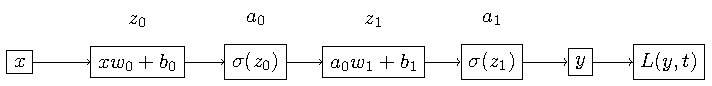
\includegraphics[width=\textwidth]{tikzfigures/forward.pdf}\\
        \end{center}
        In backpropagation, to compute the derivative of the loss function with respect to a specific 
        weight (e.g., $w_0$), it is necessary to trace the path of influence of that weight through all 
        the functions in the network. This is done by applying the chain rule in a reverse manner, 
        starting from the output layer back to the input layer.
        \begin{center}
            Backward Pass\\
            \hspace{1cm}
            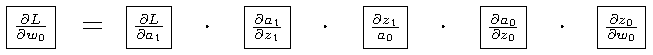
\includegraphics[width=\textwidth]{tikzfigures/backwards.pdf}
        \end{center}
        \caption{Illustration of the Chain Rule in Forward and Backward Passes}\label{fig:chainrule}
    \end{figure}

    Key Concepts in Backpropagation:

    \begin{itemize}
        \item \textbf{Forward Pass:} In the forward pass, inputs are passed through the network, layer by layer, 
            to compute the output. Each node's output is a function of its inputs, which are the outputs of 
            nodes in the previous layer.

        \item \textbf{Backward Pass:} The backward pass is where backpropagation is applied. After computing 
            the loss (the difference between the predicted output and the actual output), we propagate 
            this loss backward through the network. This involves applying the chain rule to compute partial 
            derivatives of the loss with respect to each weight in the network.

        \item \textbf{Gradient Descent:} The gradients computed through backpropagation are used to update 
            the weights of the network. This is typically done using gradient descent or one of its variants, 
            where the weight update is proportional to the negative gradient, aiming to minimize the loss function.

        \item \textbf{Activation Functions:} The role of activation functions in each neuron is crucial. 
            They introduce non-linearities into the model, allowing neural networks to learn complex patterns. 
            Derivatives of these activation functions play a significant role in the backpropagation process.
    \end{itemize}

    By iteratively performing forward and backward passes and updating the model parameters using gradient descent, 
    neural networks can effectively learn from data. Backpropagation is thus a cornerstone technique in 
    neural network training, enabling these models to capture and learn from complex patterns in data.




\section{Neural Networks}
\label{sec:NN}

    Neural networks extend the principles of logistic regression to more complex architectures, enabling the 
    modeling of a wider range of nonlinear relationships. At their core, neural networks can be conceptualized 
    as a series of logistic regression models interconnected in a network structure. This similarity allows for a 
    degree of code reusability across logistic regression, linear regression, and neural network implementations.

    \begin{figure}[h]
        \begin{center}
            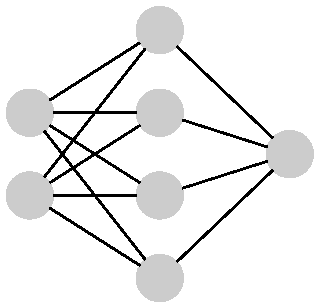
\includegraphics[width=0.4\textwidth]{tikzfigures/nn.pdf}
        \end{center}
        \caption{A model of a neural network with one hidden layer consisting of four nodes}\label{fig:nn}
        \cite{neutelings_tikzcode}
    \end{figure}

    \begin{figure}[h]
        \begin{center}
            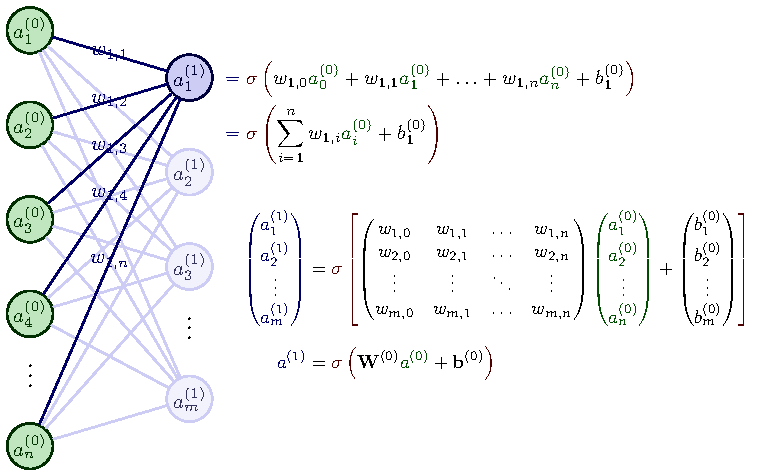
\includegraphics[width=0.9\textwidth]{tikzfigures/nnActivation.pdf}
        \end{center}
        \caption{Illustration of how a single node gets its value during a forward pass. This shows that matrix 
        operations can be used for more efficient calculations. When $a$ is a batch of inputs, these calculations 
    become matrix-matrix multiplications, significantly speeding up both training and inference.}\label{fig:nn_math}   
        \cite{neutelings_tikzcode}
    \end{figure}

    One of the defining features of neural networks is the use of activation functions. These functions introduce 
    non-linearity into the model, allowing the network to learn complex patterns. Common examples of activation 
    functions include the sigmoid, tanh, and ReLU functions. Each has unique characteristics that make them suitable 
    for different types of neural network architectures.
    In a neural network with no hidden layers, the model essentially becomes a linear regression model, represented by 
    the equation $y = x_0w_0 + x_1w_1 + x_2w_2 + ... + x_nw_n + b_0$. By introducing an activation function at the 
    output layer, the model transforms into a logistic regression model, suitable for binary classification tasks. 
    The flexibility of neural networks arises from their ability to incorporate multiple hidden layers with a variety 
    of activation functions, enabling them to capture complex relationships in data.
    Backpropagation is the mechanism through which neural networks learn. By calculating the derivatives of the loss 
    function with respect to the network's parameters, backpropagation allows for the adjustment of these parameters 
    in a way that minimizes the loss. This process is essential for training neural networks and is applicable across 
    different network architectures, from simple single-layer networks to deep, multi-layered structures.
    To summarize, neural networks are a powerful extension of logistic and linear regression models, capable of 
    handling a broad spectrum of tasks from simple regression to complex pattern recognition. Their versatility and 
    adaptability, combined with the efficiency of matrix operations, make them a cornerstone technology in the field 
    of machine learning.



\section{Data}
\label{sec:data}

    For our classification task, we will utilize the widely recognized Wisconsin Breast Cancer 
    Dataset\cite{misc_breast_cancer17}. This dataset comprises 569 data points, 
    each with 30 distinctive features. 
    These features are derived from digitized images of a fine needle aspirate (FNA) of breast masses, focusing on 
    various characteristics of the cell nuclei depicted in the images.
    The dataset quantifies several attributes for each cell nucleus, including radius, texture, perimeter, area, 
    smoothness, compactness, concavity, concave points, symmetry, and fractal dimension. For each attribute, three 
    types of measurements are provided: the mean, standard error, and the "worst" or largest (which represents the 
    mean of the three largest values). This results in a total of 30 features for each data point. For instance, 
    field 1 represents the Mean Radius, field 11 is Radius SE, and field 21 corresponds to the Worst Radius.
    All feature values in this dataset are recorded with four significant digits, and there are no missing attribute 
    values. The class distribution within the dataset is as follows: 357 benign cases and 212 malignant cases.
    The primary objective is to classify these tumors as either benign or malignant based on the features provided. 
    In this context, a positive result indicates a benign tumor, while a negative result signifies a malignant tumor. 
    Essentially, our goal is to accurately identify cases of cancer and classify them as negative.


    \begin{figure}[h]
        \begin{center}
            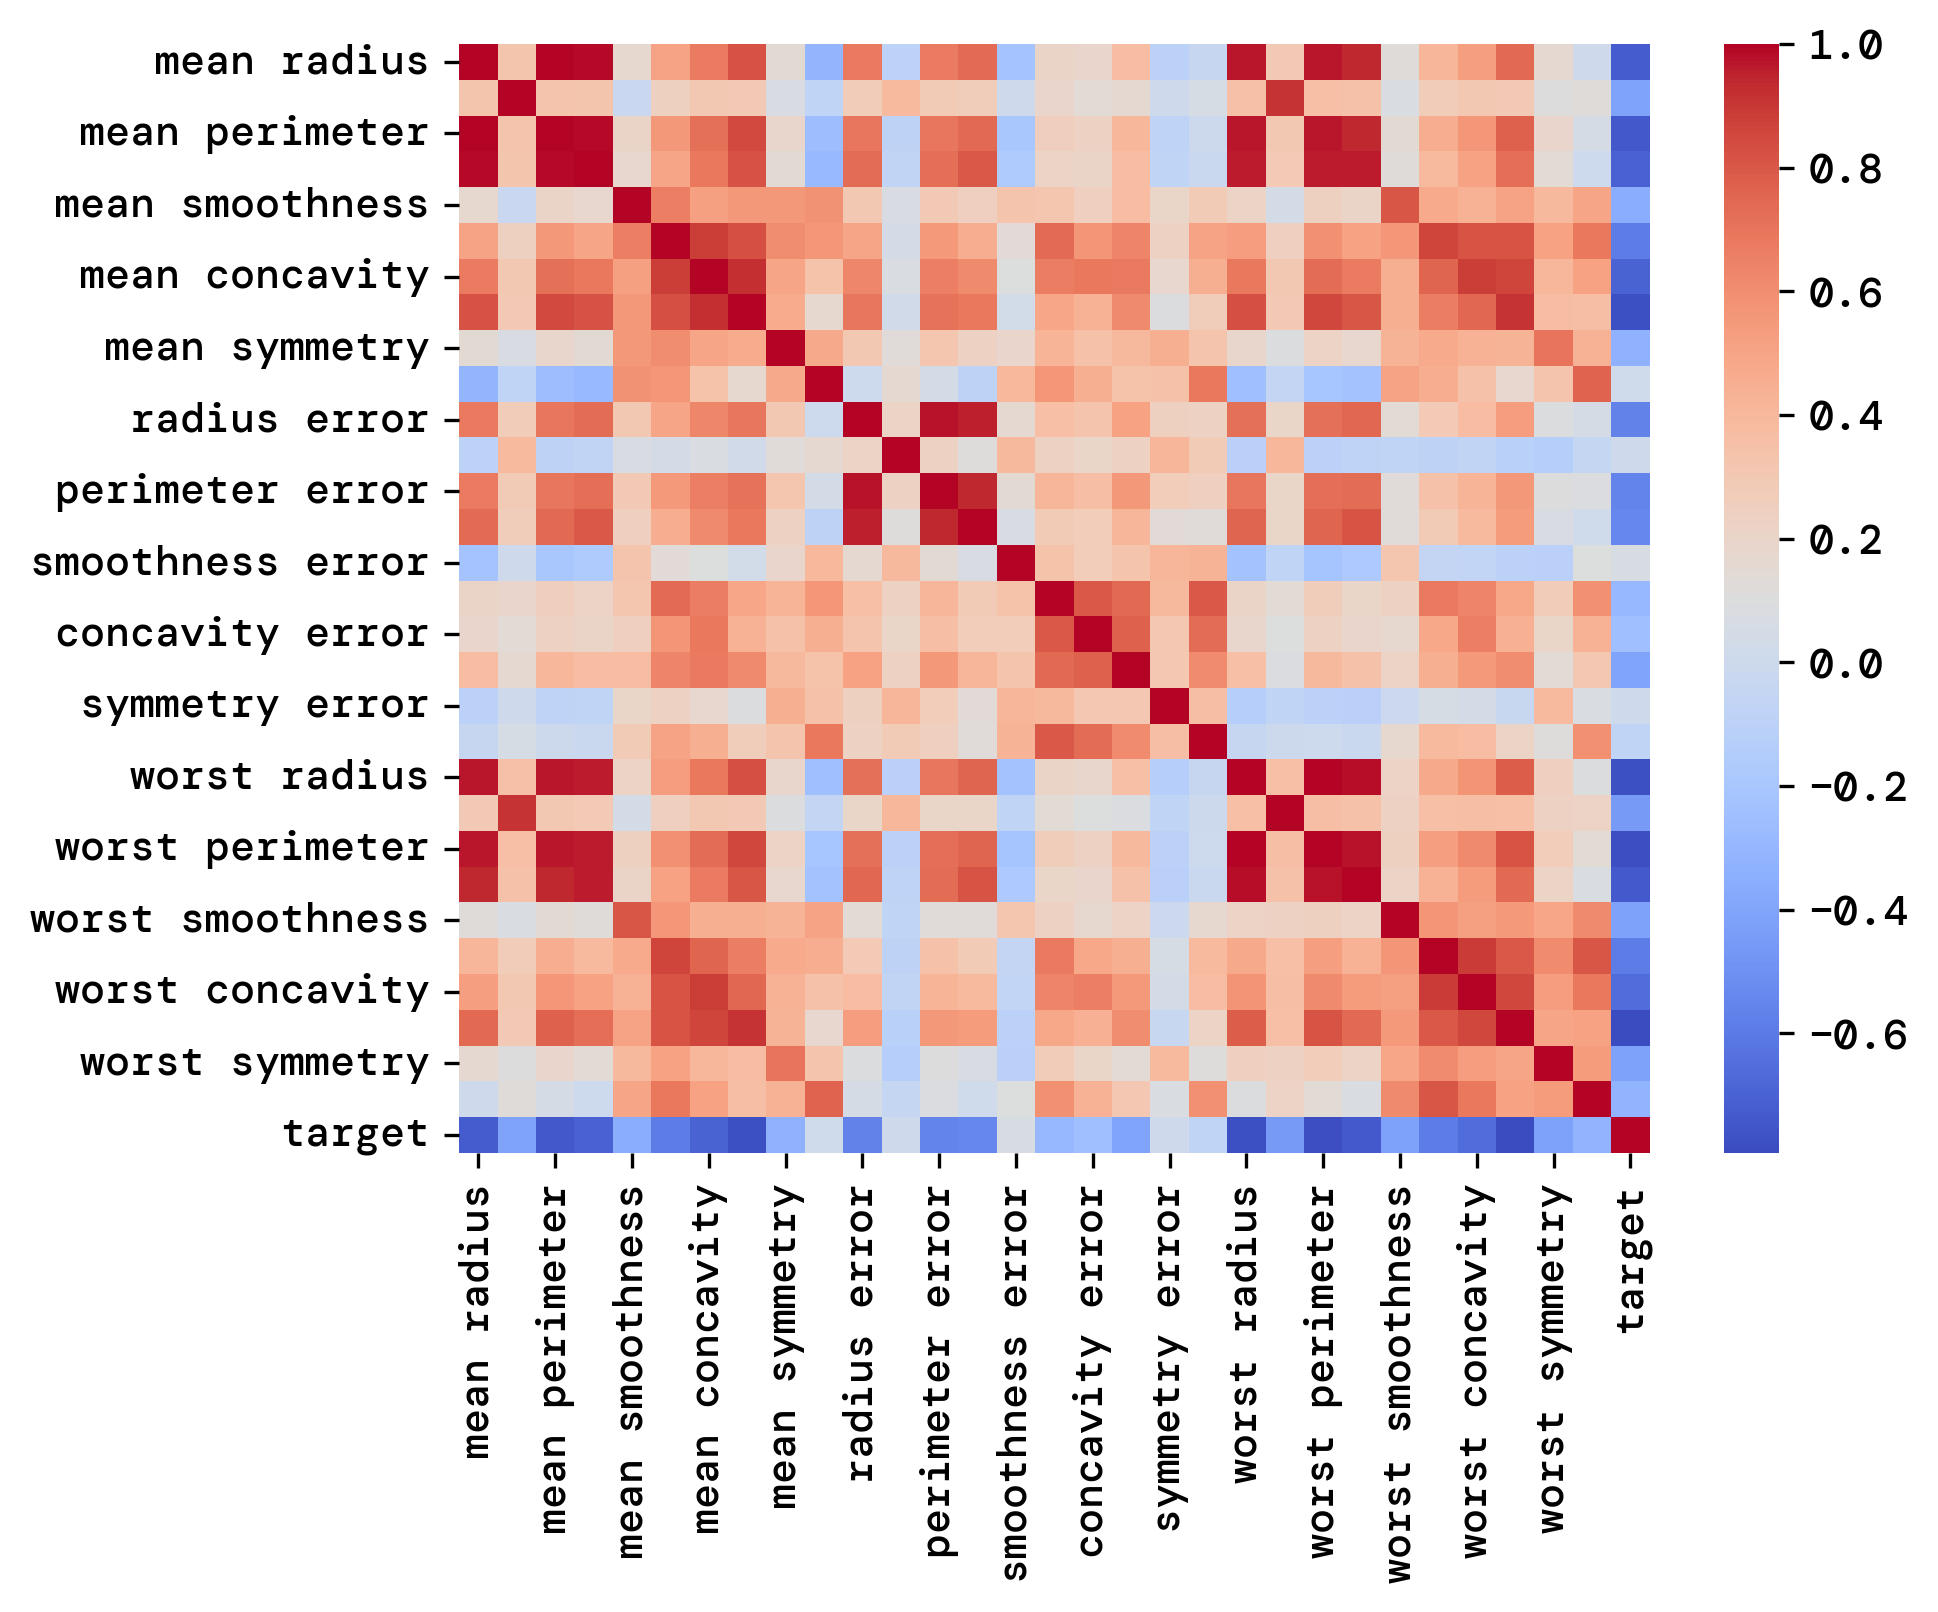
\includegraphics[width=0.8\textwidth]{../runsAndFigures/feature_correlation.png}
        \end{center}
        \caption{Feature correlation matrix. This provides insight into the redundancy among features. 
        Only every other feature is annotated, but the missing labels can be inferred from 
            Figure~\ref{fig:feature_histogram}.}\label{fig:feature_correlation}
    \end{figure}

    \begin{figure}
        \begin{center}
            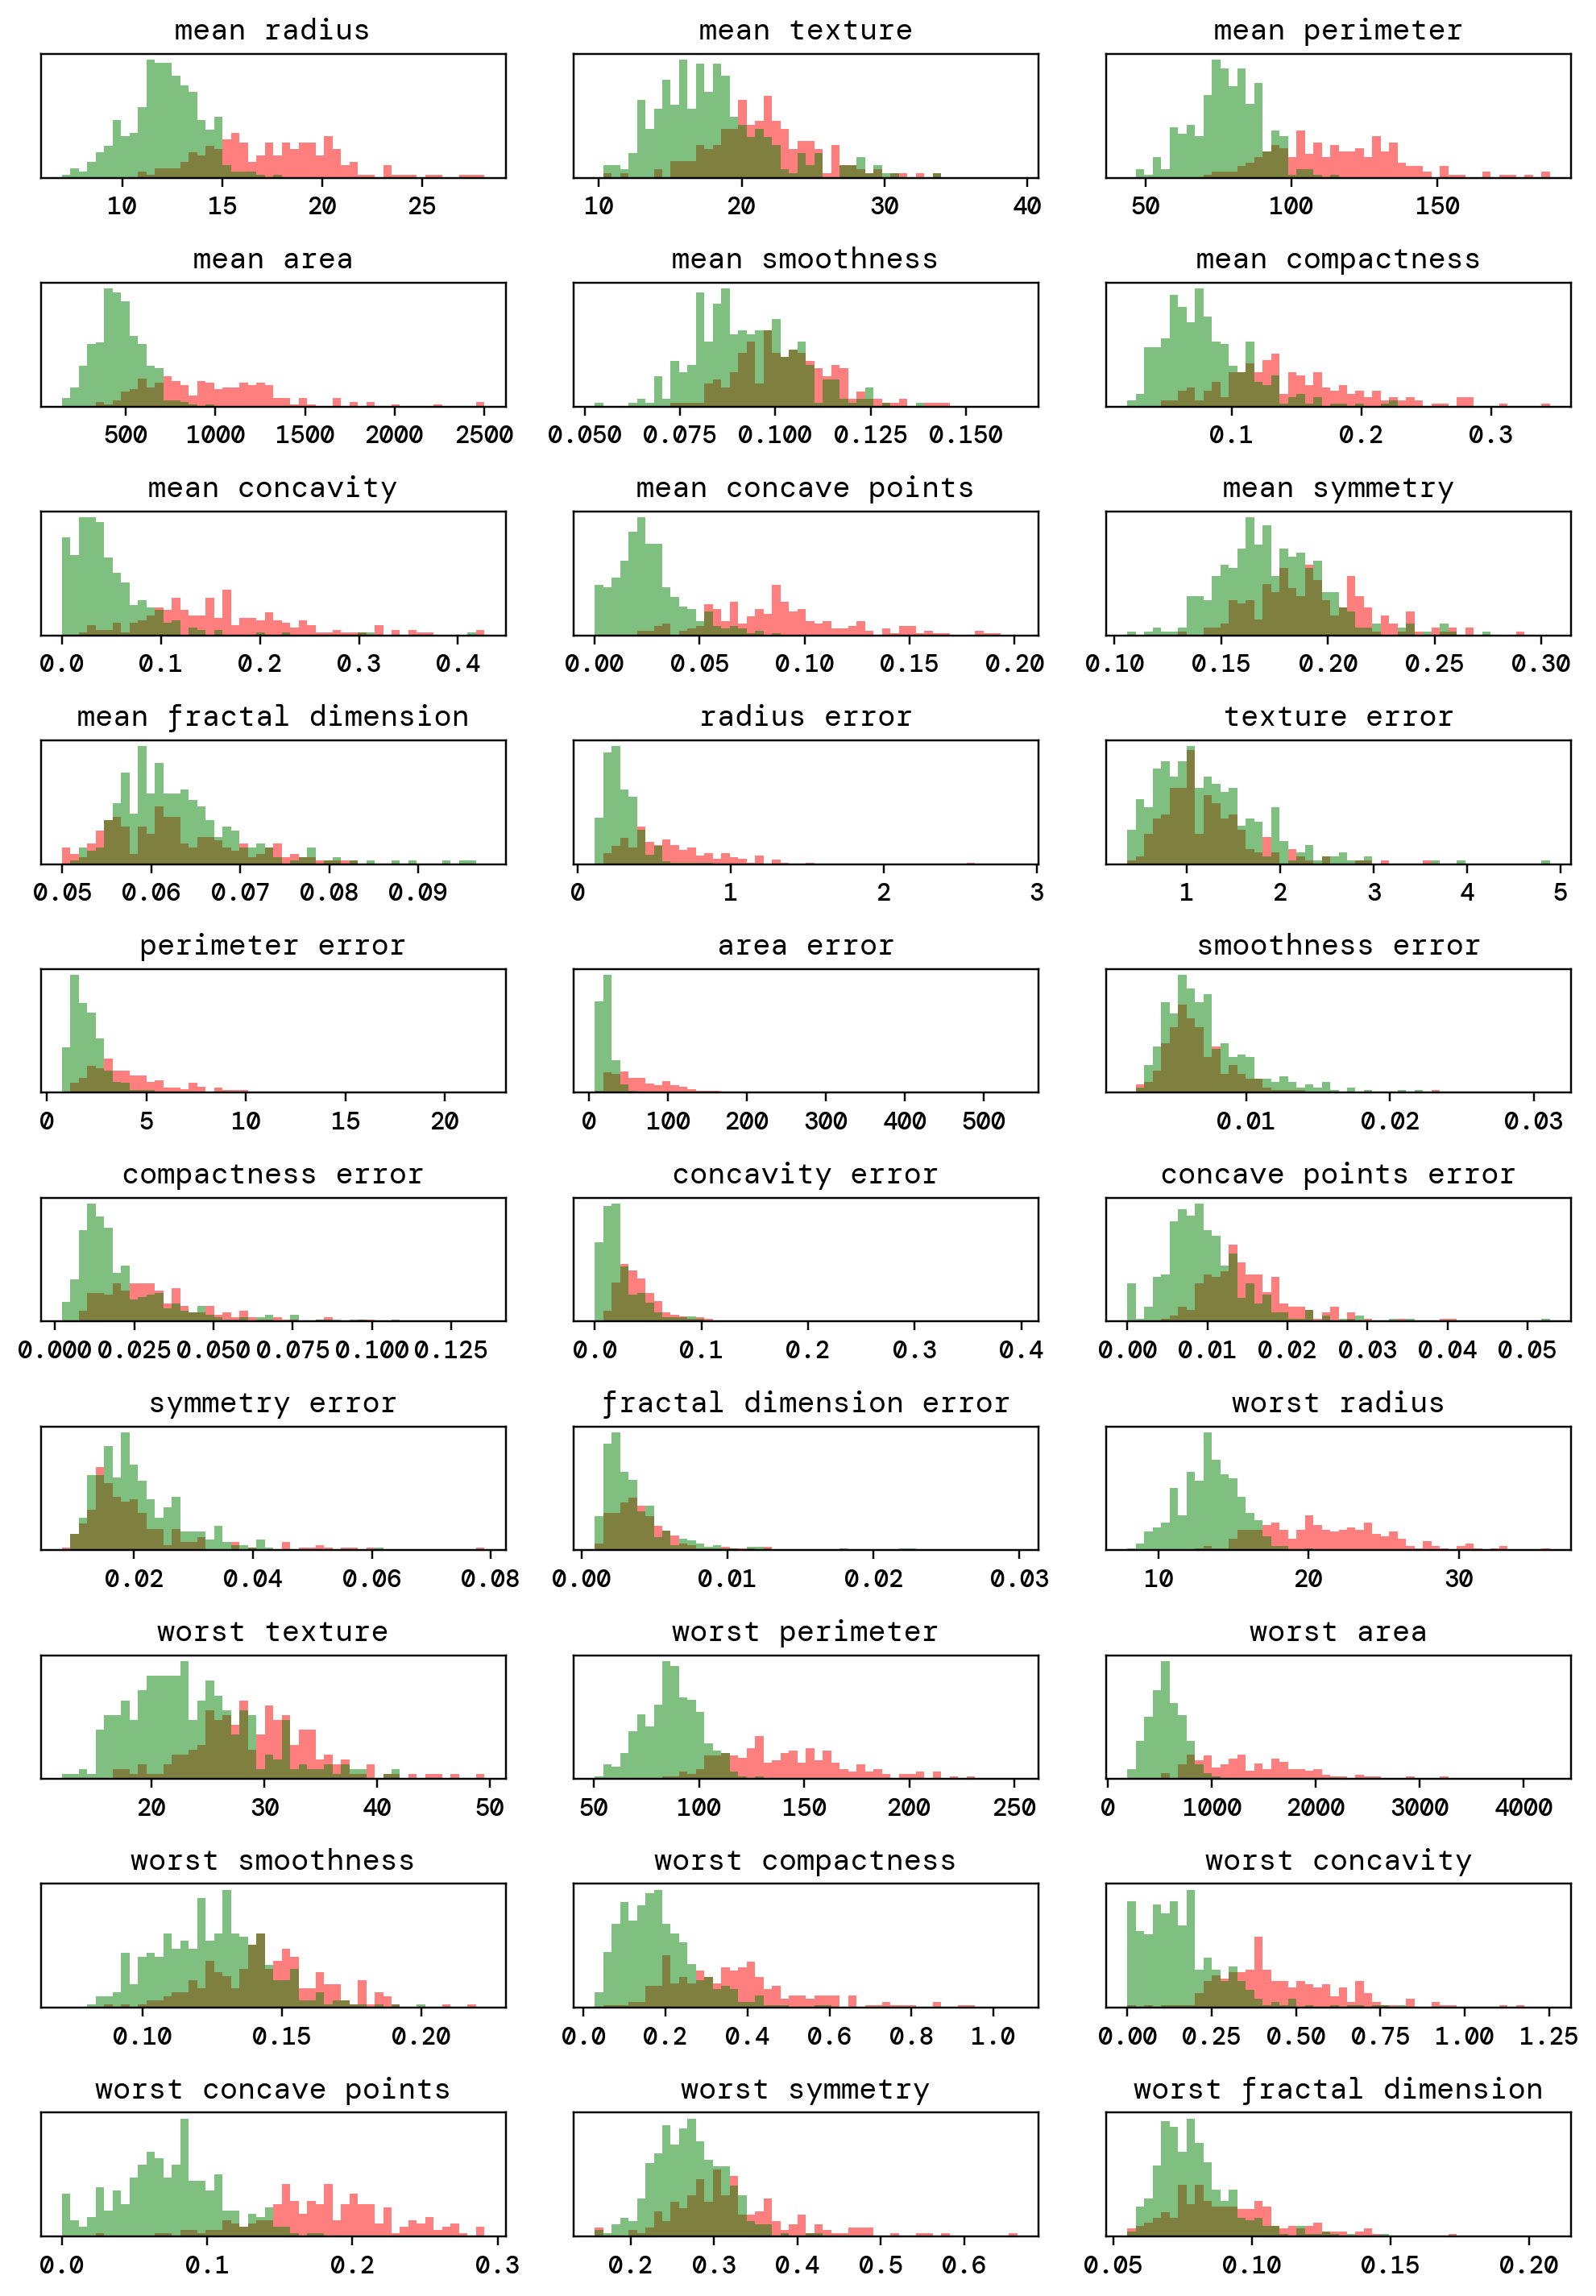
\includegraphics[width=0.95\textwidth]{../runsAndFigures/feature_histogram.png}
        \end{center}
        \caption{Feature histogram. The red class ($0$) represents malignant cases, while the green class 
        ($1$) indicates benign cases.}\label{fig:feature_histogram}
    \end{figure}


\clearpage

\section{Results and Analysis}
\label{sec:resultsdiscussion}

    In our experiments, we employed the cross-entropy loss function, The gradient of the loss function 
    with respect to the model's parameters was computed using automatic differentiation. 
    We used the SKLearn\cite{scikit-learn}
    library to perform cross-validation for a more robust evaluation of our models.
    We used k-fold cross-validation with $k=6$ folds. The results presented in this section are based on
    the average of the results from the 6 folds. The bar plots show also show the standard deviation of the
    results from the 6 folds.
    During our hyperparameter tuning phase, we observed interdependencies between certain hyperparameters. Notably, 
    the learning rate and the number of epochs showed a significant correlation, as did the batch size and the learning 
    rate. Such dependencies imply that these hyperparameters cannot be optimized independently for the most effective 
    training process. Ideally, a comprehensive grid search across multiple dimensions of hyperparameters would be 
    conducted. However, due to constraints in time and computational resources, our experiments were limited.
    We were able to conduct grid searches, but these were restricted to two dimensions at most. While this limitation 
    prevented a thorough exploration of the hyperparameter space, the results from these partial grid searches provided 
    valuable insights. They served as indicators, pointing us towards regions in the hyperparameter space where optimal 
    settings might exist.
    The analysis of these results suggests that while we have identified promising hyperparameter settings, a more 
    exhaustive search might yield further improvements. 

\subsection{Hyperparameters}
\label{sec:hyperparameters}

    \begin{figure}[!ht]
        \begin{minipage}[t]{0.5\textwidth - 1mm}
            \begin{center}
                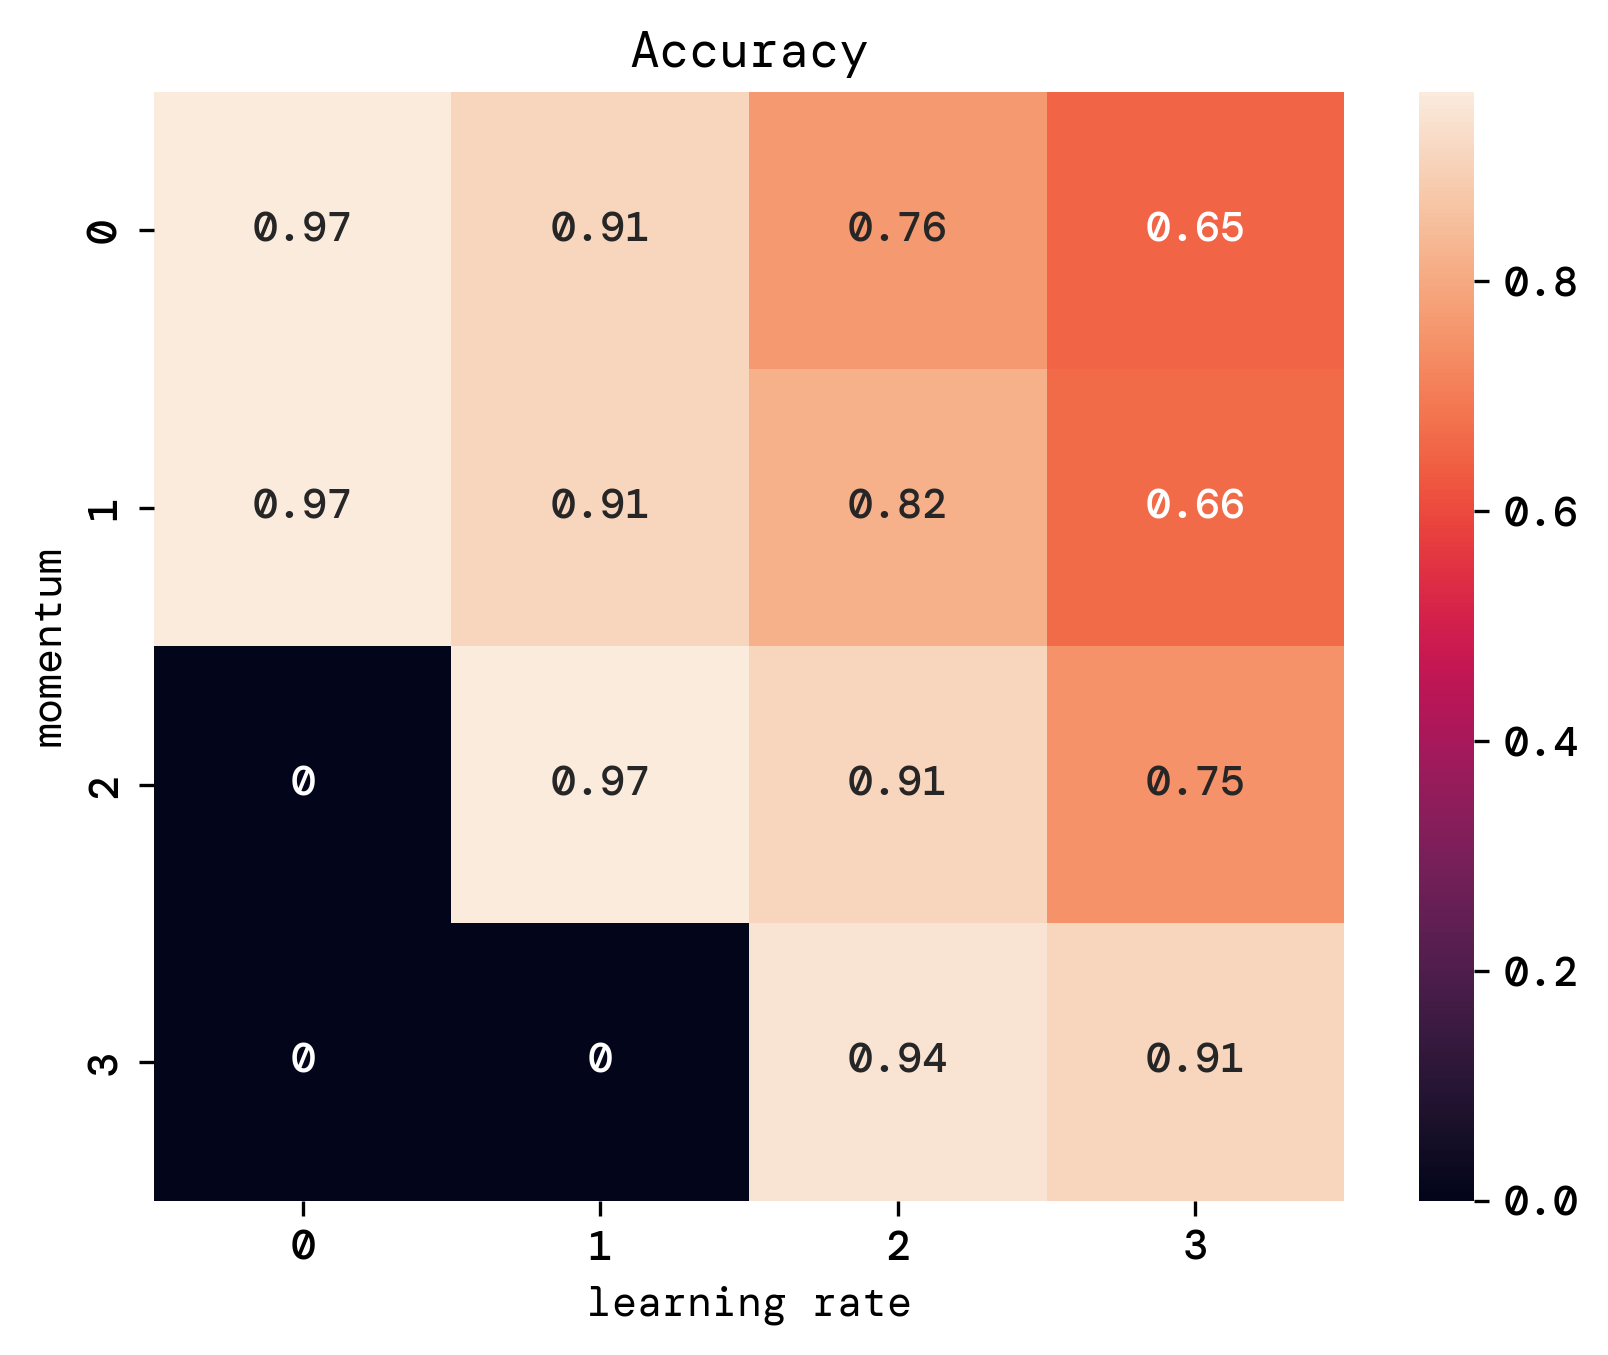
\includegraphics[width=\textwidth]{../runsAndFigures/accuracy_lr_gamma.png}
            \end{center}
            \caption
            {
                Accuracy versus learning rate and momentum.
            }\label{fig:accuracy_lr_gamma}
        \end{minipage}
        \hspace{2mm}
        \begin{minipage}[t]{0.5\textwidth - 1mm}
            \begin{center}
                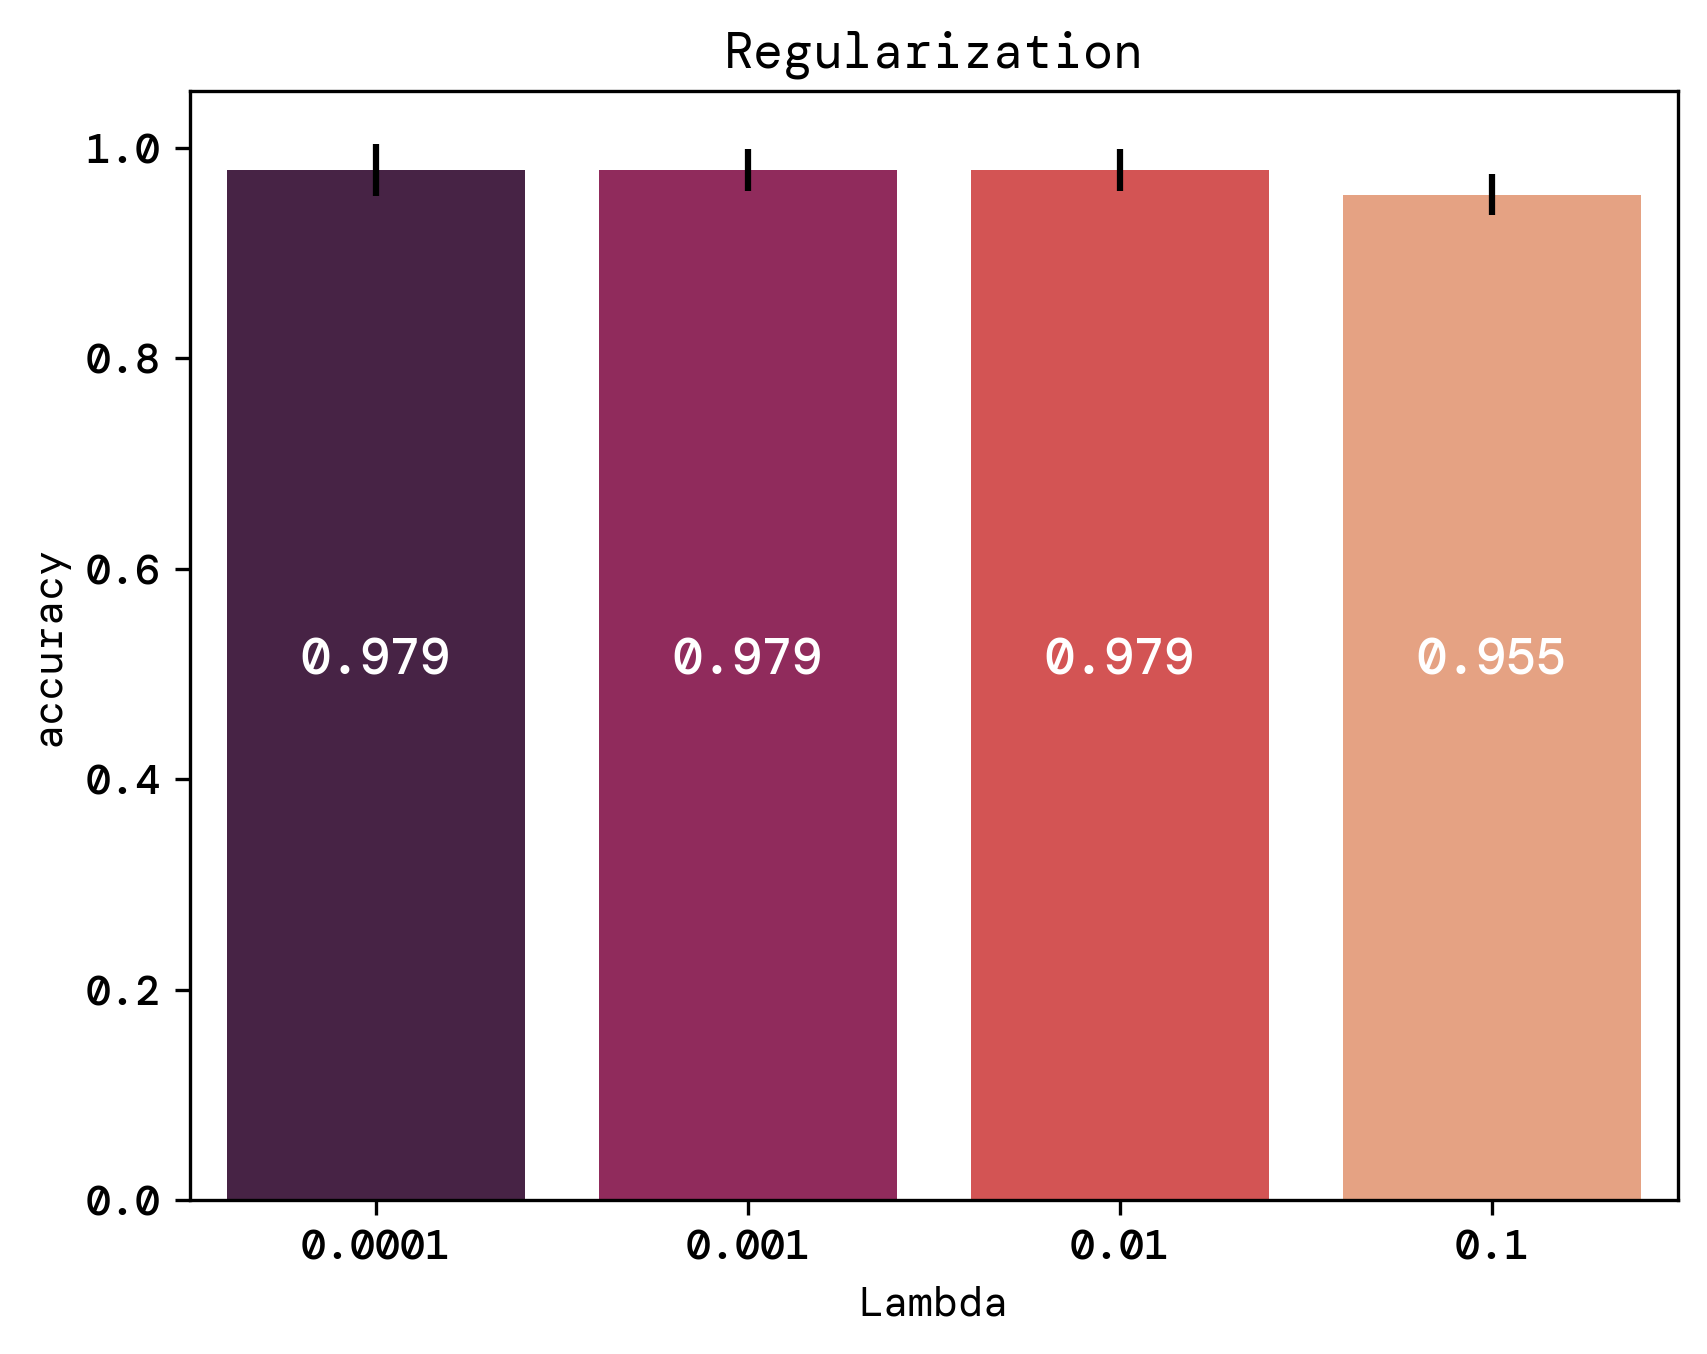
\includegraphics[width=\textwidth]{../runsAndFigures/accuracy_alpha.png}
            \end{center}
            \caption
            {
                Accuracy versus regualarization.
            }\label{fig:accuracy_aplha}
        \end{minipage}
    \end{figure}

    Our findings indicate that incorporating momentum is beneficial, particularly with a value of 
    around 0.9, which emerged as the most effective in our tests. This momentum allows for a higher learning rate, 
    enhancing the training process. In contrast, excessive regularization seems to adversely affect model performance.
    
    \begin{figure}[ht]
        \begin{minipage}[t]{0.5\textwidth - 1mm}
            \begin{center}
                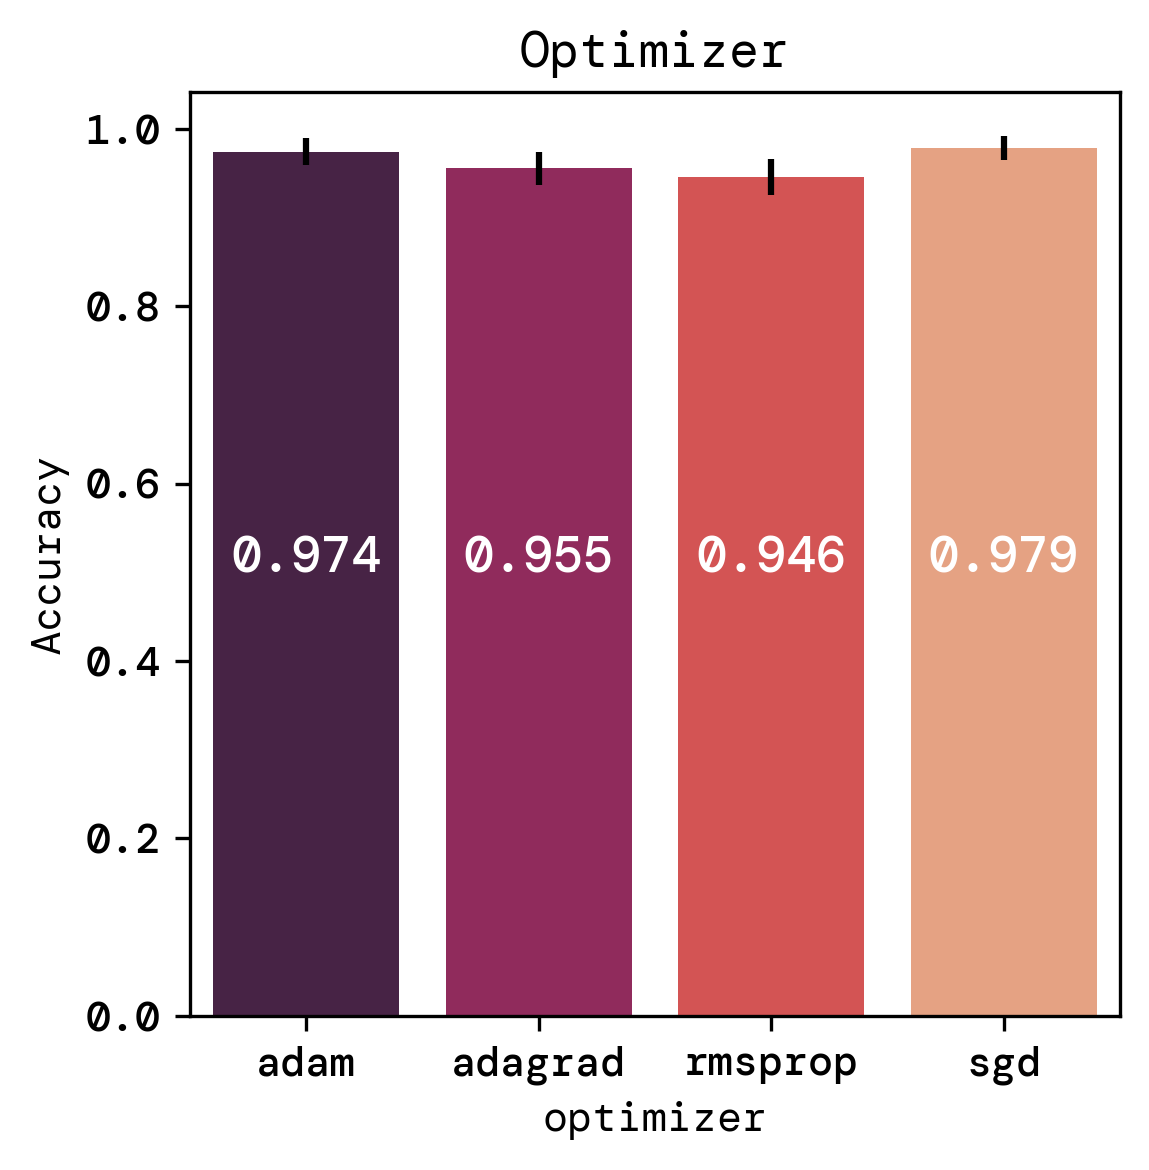
\includegraphics[width=\textwidth]{../runsAndFigures/accuracy_optimizer.png}
            \end{center}
            \caption
            {
                Model accuracy across different optimizers.
            }\label{fig:accuracy_optimizer}
        \end{minipage}
        \hspace{2mm}
        \begin{minipage}[t]{0.5\textwidth - 1mm}
            \begin{center}
                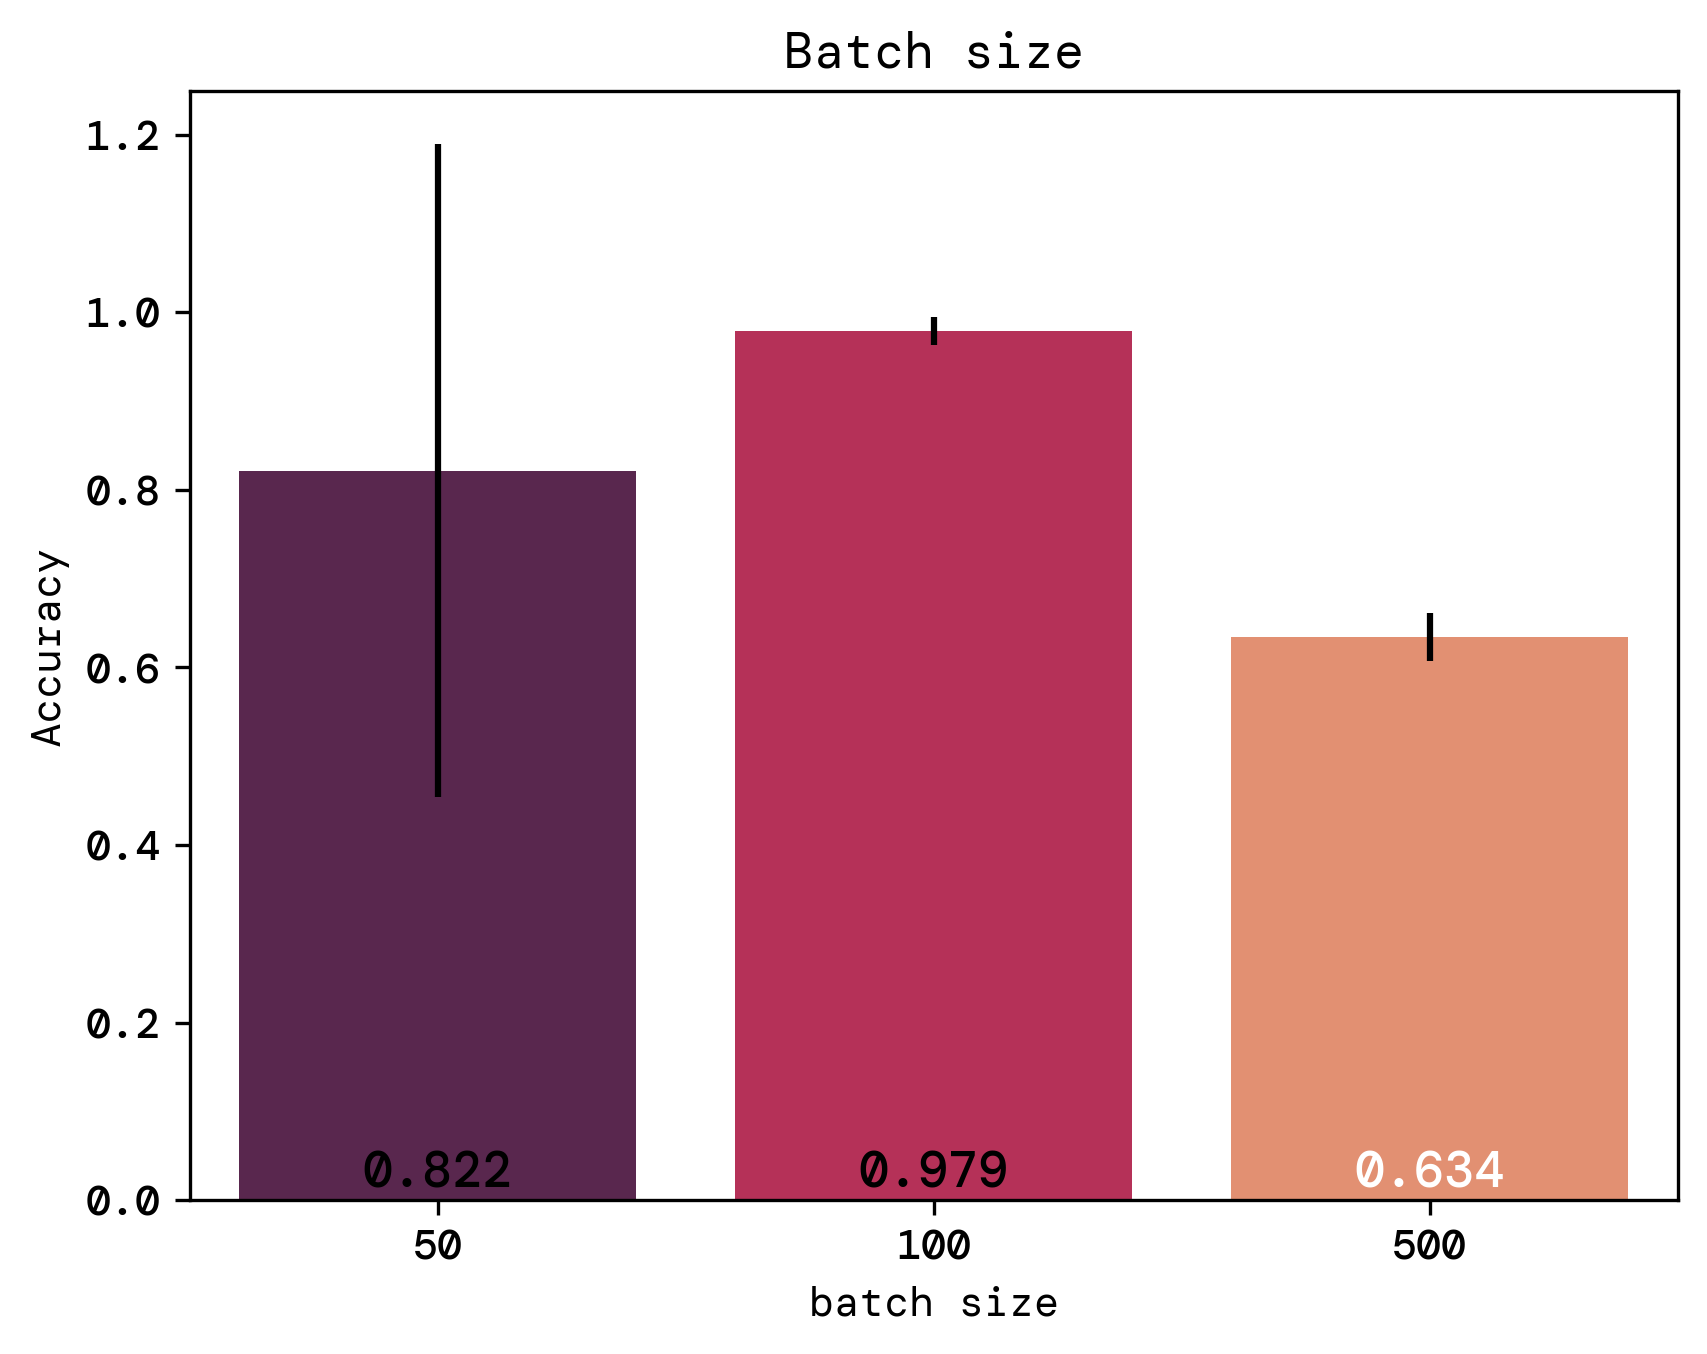
\includegraphics[width=\textwidth]{../runsAndFigures/accuracy_batch.png}
            \end{center}
            \caption
            {
                Accuracy based on batch size.
            }\label{fig:accuracy_batch}
        \end{minipage}
    \end{figure}

    The choice of optimizer did not significantly impact the model's performance. However, 
    Adam optimizer showed a slight advantage over others. The batch size also played a role, 
    with certain sizes yielding better accuracy.



    \begin{figure}[!ht]
        \begin{minipage}[t]{0.5\textwidth - 1mm}
            \begin{center}
                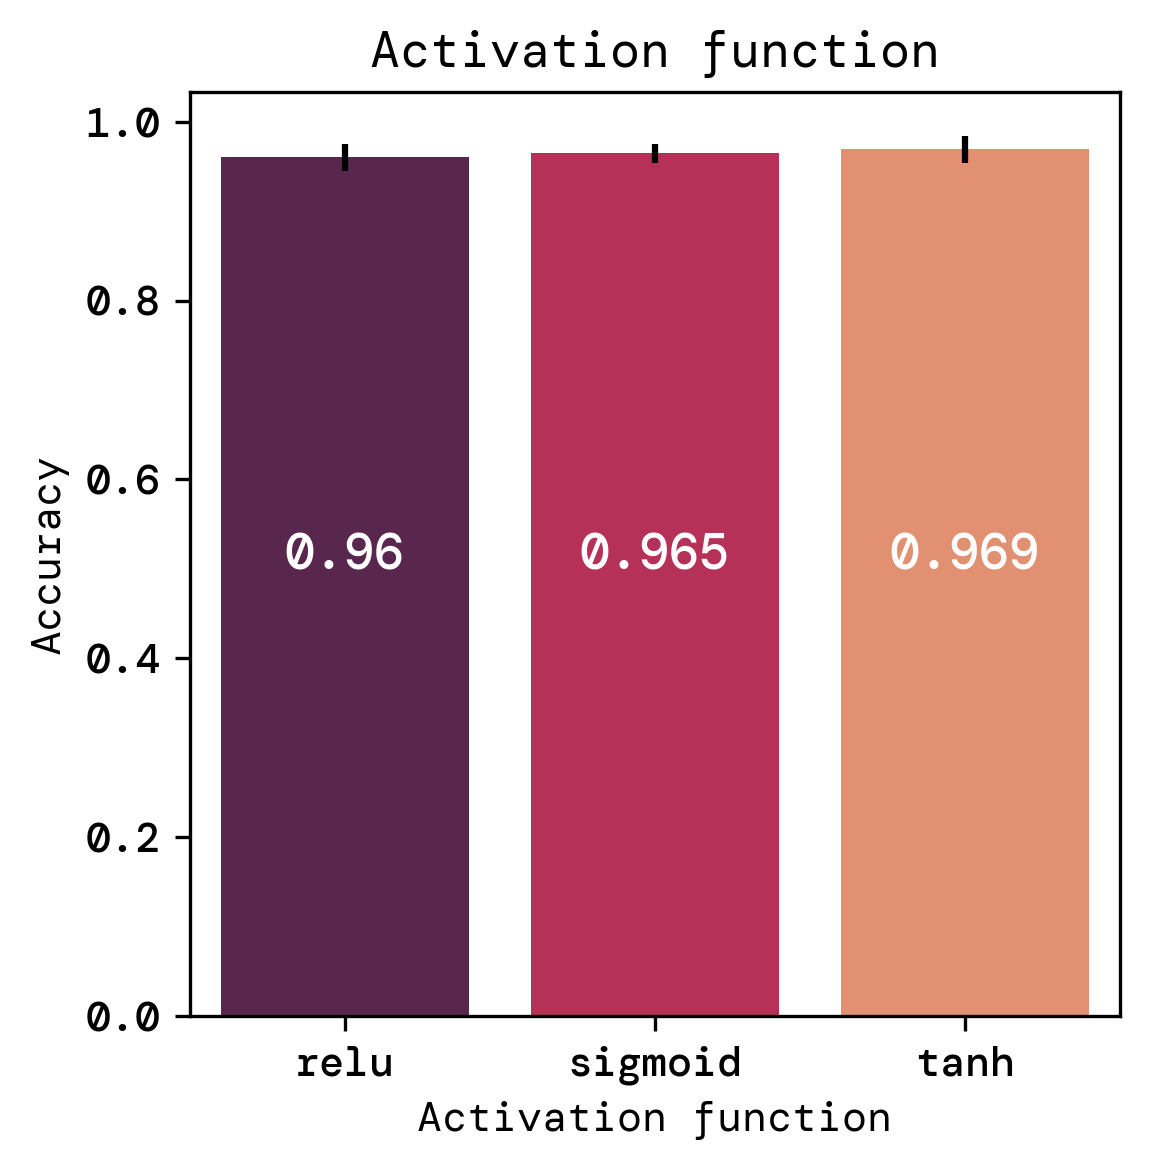
\includegraphics[width=\textwidth]{../runsAndFigures/accuracy_activ.png}
            \end{center}
            \caption
            {
                Model performance with different activation functions.
            }\label{fig:accuracy_activ}
        \end{minipage}
        \hspace{2mm}
        \begin{minipage}[t]{0.5\textwidth - 1mm}
            \begin{center}
                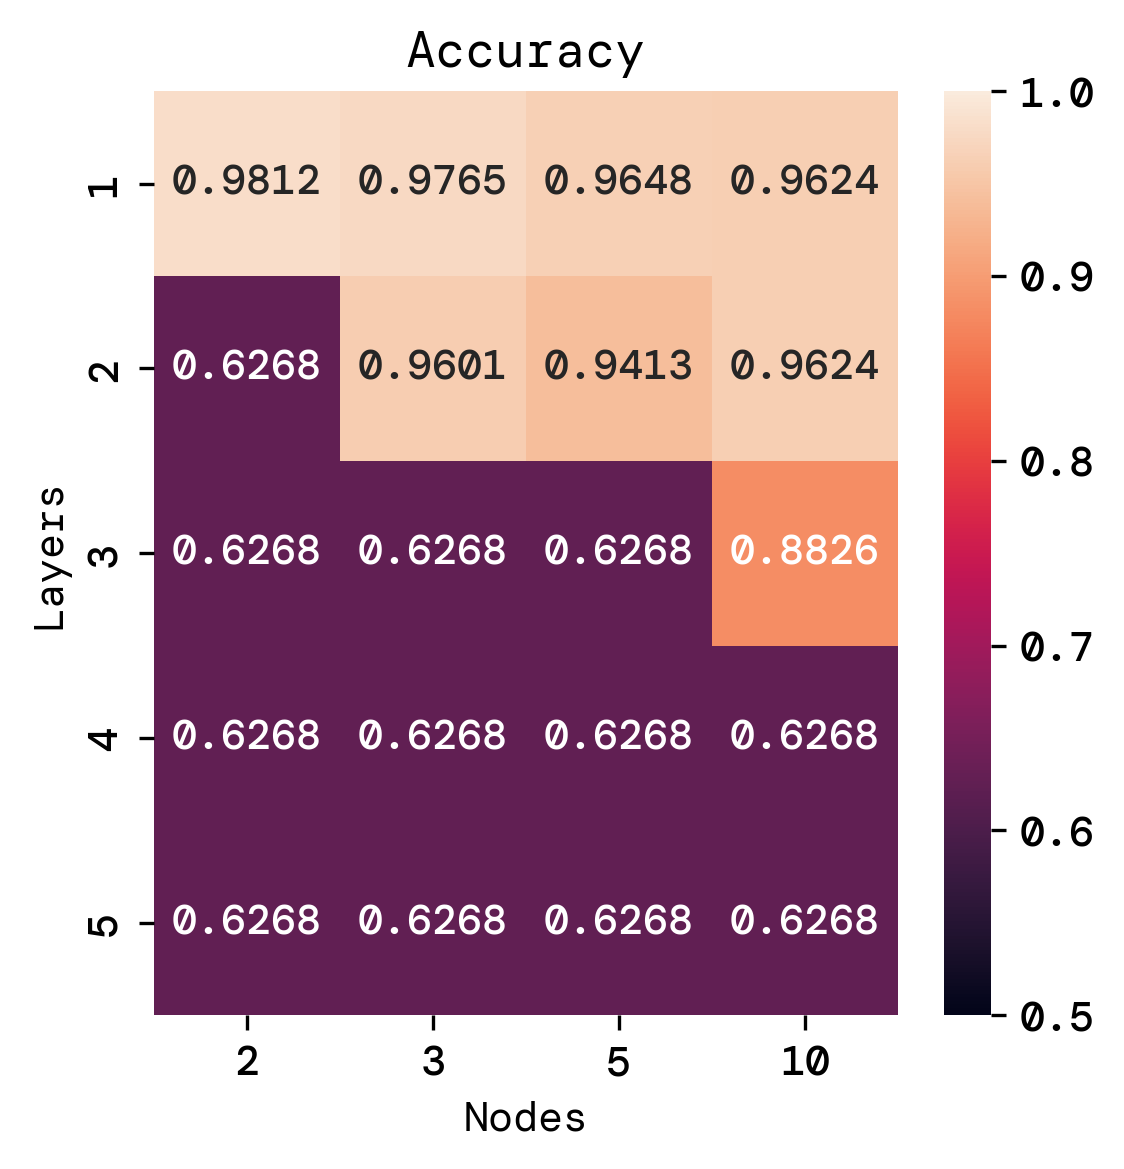
\includegraphics[width=\textwidth]{../runsAndFigures/accuracy_layers_nodes.png}
            \end{center}
            \caption
            {
                Accuracy in relation to the number of layers and nodes.
            }\label{fig:accuracy_layers_nodes}
        \end{minipage}
    \end{figure}



    In summary, our results highlight the importance of momentum in the learning process and suggest that 
    over-regularization can be detrimental. The choice of optimizer and batch size, while not as critical, 
    still influences model performance, with the Adam optimizer slightly outperforming others. The findings 
    underscore the need for careful hyperparameter tuning in


\subsection{Final Evaluation and Comparisons}
\label{sec:comparisons}


\begin{figure}[h]
        \begin{center}
            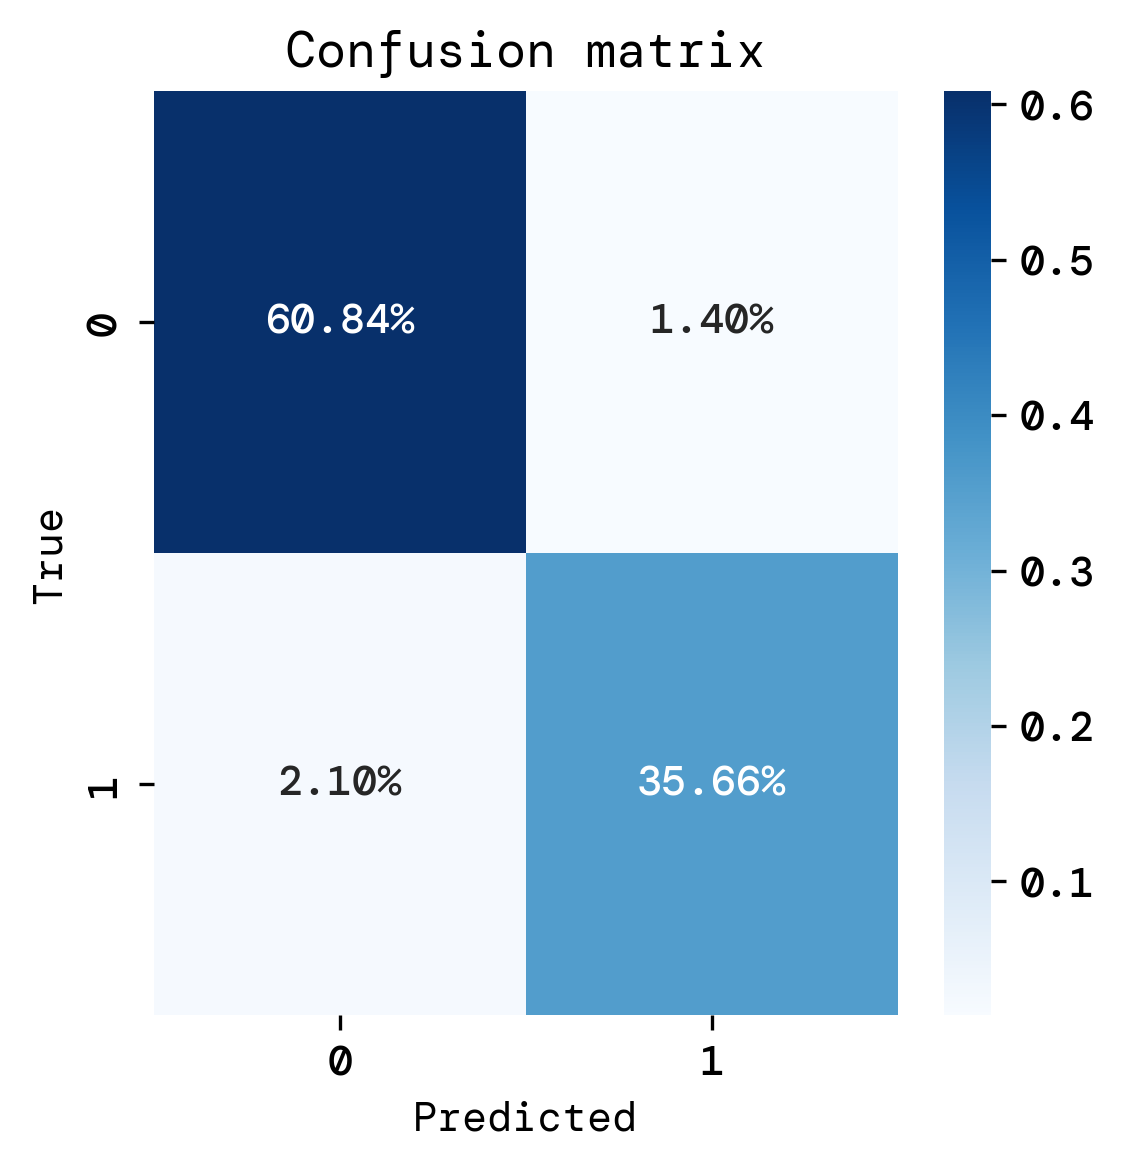
\includegraphics[width=0.5\textwidth]{../runsAndFigures/confusion_matrix.png}
        \end{center}
        \caption
        {
            Confusion matrix for the best model. 
            The model has an accuracy of 96\% on the test set.
        }\label{fig:confusion_matrix}
    \end{figure}



\section{Conclusion}
\label{sec:conclusion}






















% \acks{}


\clearpage 

\appendix
\renewcommand{\theHchapter}{appendix\Alph{chapter}}
\renewcommand{\theHsection}{appendix\thesection}

\phantomsection
\addcontentsline{toc}{chapter}{Appendix}


\chapter*{Appendix A}
\label{app:appendixA}


\section{Regression with Neural Networks}
\label{sec:regression}

    In our previous project\cite{MachineLearningProjects_2023}, we explored the fitting of linear models and 
    polynomials to data, deriving optimal parameters \(\beta\) through an analytical approach. 
    This method demonstrated that, theoretically, polynomials can approximate any function, given a sufficiently 
    high degree of freedom. However, this approach has practical limitations. 
    Providing a model with infinite degrees of freedom is not feasible due to computational constraints 
    and the risk of overfitting. How can we approximate complex functions without resorting to high-degree 
    polynomials? A promising solution is to construct models that are not based on a single high-degree polynomial 
    but are instead composed of simpler, interconnected components. This is where neural networks come into play.
    Neural networks offer a flexible architecture that can approximate a wide range of functions. By 'gluing together' 
    multiple simple functions, such as linear segments in the case of basic neural networks, they can model complex 
    relationships in the data. Unlike polynomials, neural networks are not limited to a specific functional form and 
    can be adapted for both regression and classification tasks. Their layered structure, where each layer can learn 
    different aspects of the data, allows them to capture both simple and intricate patterns.

    Thus, neural networks provide a powerful and versatile alternative to polynomial regression, capable of handling 
    diverse data modeling challenges, as we will explore in this section.



\section*{Data}

    For regression we will be using perlin noise to generate our dataset 

    \begin{figure}
        \begin{center}
            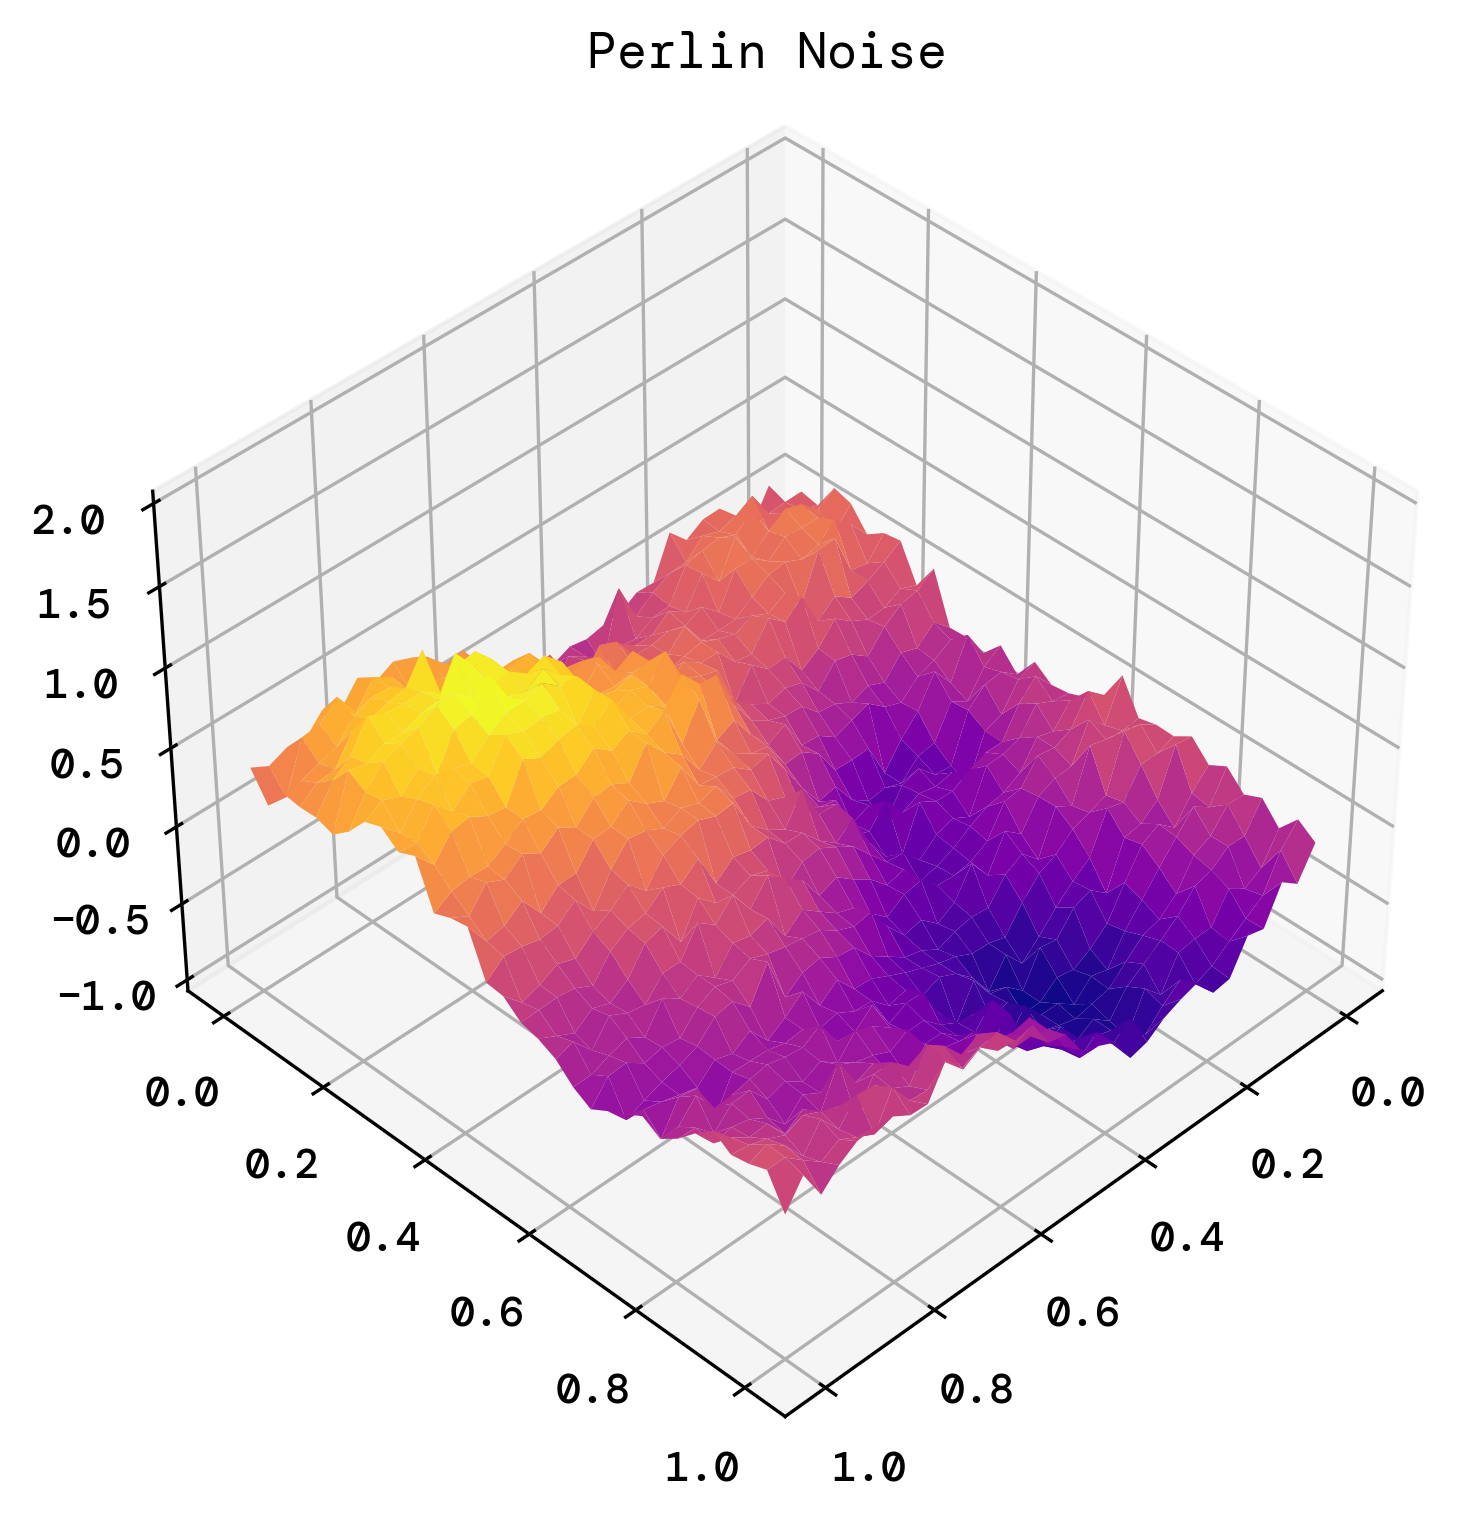
\includegraphics[width=0.5\textwidth]{../runsAndFigures/perlinNoise.png}
        \end{center}
        \caption{}\label{fig:perlin}
    \end{figure}

    Solving a regression problem with linear regression and neural networks using gradient optimization.



\section*{Results and Analysis}
\label{sec:resultsdiscussion2}




\subsection*{Hyperparameters}
\label{sec:hyperparameters2}


    \begin{figure}[!ht]
        \begin{minipage}[t]{0.5\textwidth - 1mm}
            \begin{center}
                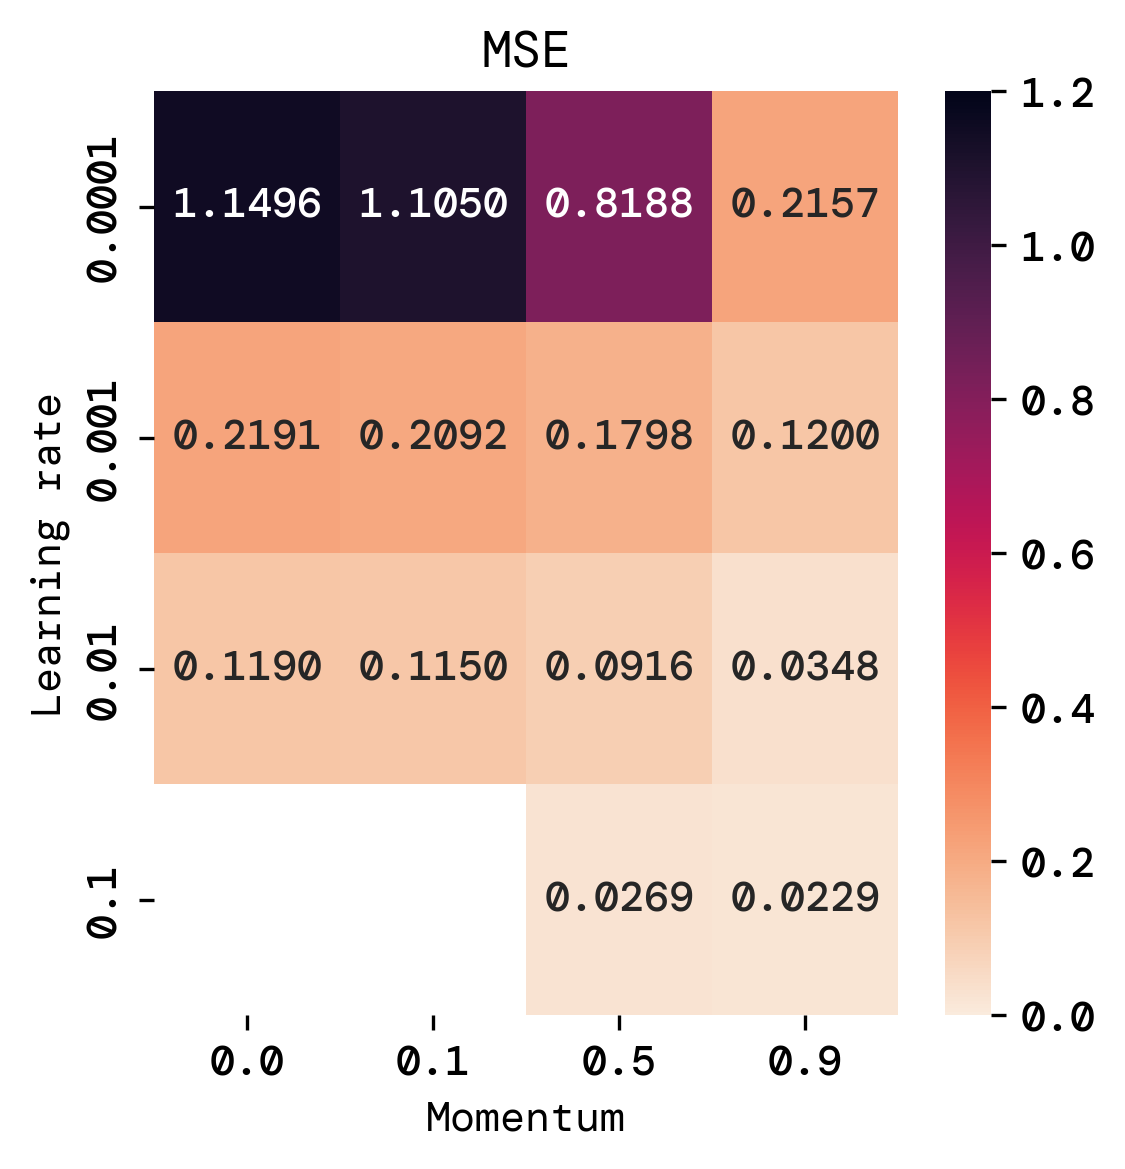
\includegraphics[width=\textwidth]{../runsAndFigures/MSE_lr_gamma.png}
            \end{center}
            \caption{In this case havving momentum seems to be beneficial. 
            We maxes out our testing range and found that 0.9 was the best value for momentum. 
            momentum allows a higher learning rate}\label{fig:MSE_lr_gamma}
        \end{minipage}
        \hspace{2mm}
        \begin{minipage}[t]{0.5\textwidth - 1mm}
            \begin{center}
                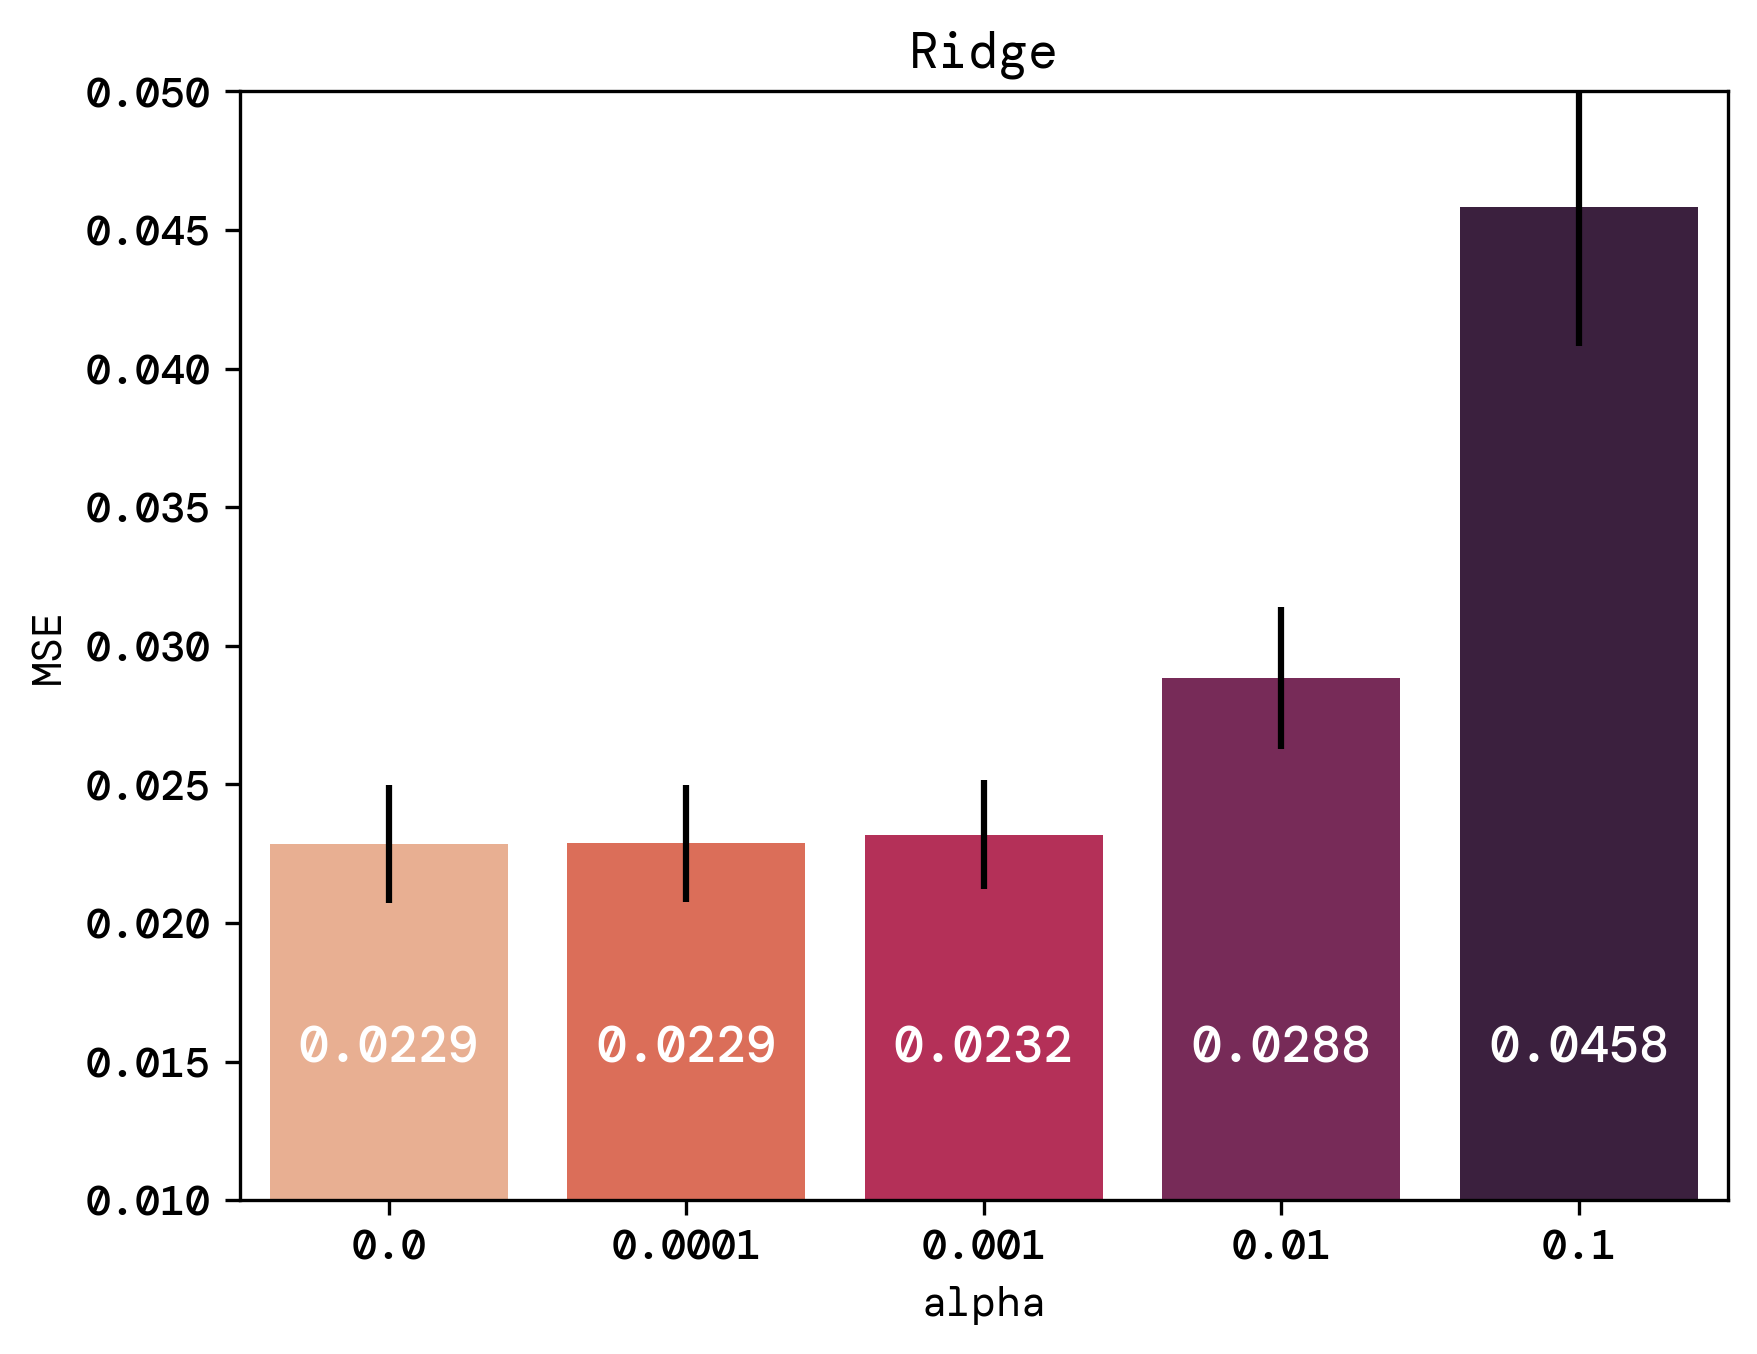
\includegraphics[width=\textwidth]{../runsAndFigures/MSE_alpha.png}
            \end{center}
            \caption{Introduction regualarization does not seem to yield any benefits, in fact
            having too much regualarization shunts performance}\label{fig:MSE_aplha}
        \end{minipage}
    \end{figure}


    \begin{figure}[!ht]
        \begin{minipage}[t]{0.5\textwidth - 1mm}
            \begin{center}
                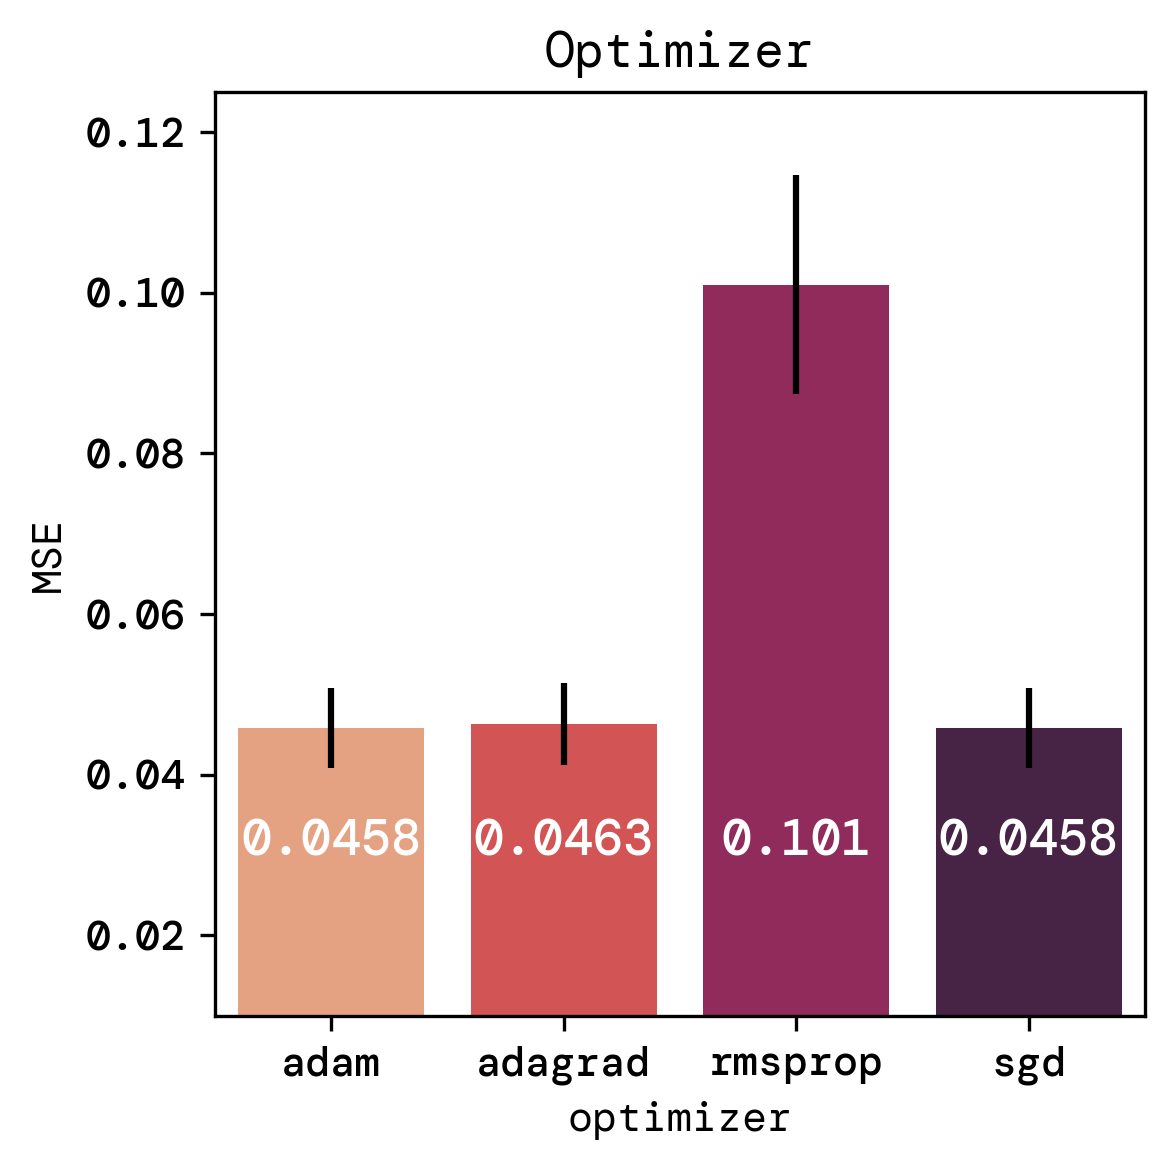
\includegraphics[width=\textwidth]{../runsAndFigures/MSE_optimizer.png}
            \end{center}
            \caption{In this case havving momentum seems to be beneficial. 
            We maxes out our testing range and found that 0.9 was the best value for momentum. 
            momentum allows a higher learning rate}\label{fig:MSE_optimizer}
        \end{minipage}
        \hspace{2mm}
        \begin{minipage}[t]{0.5\textwidth - 1mm}
            \begin{center}
                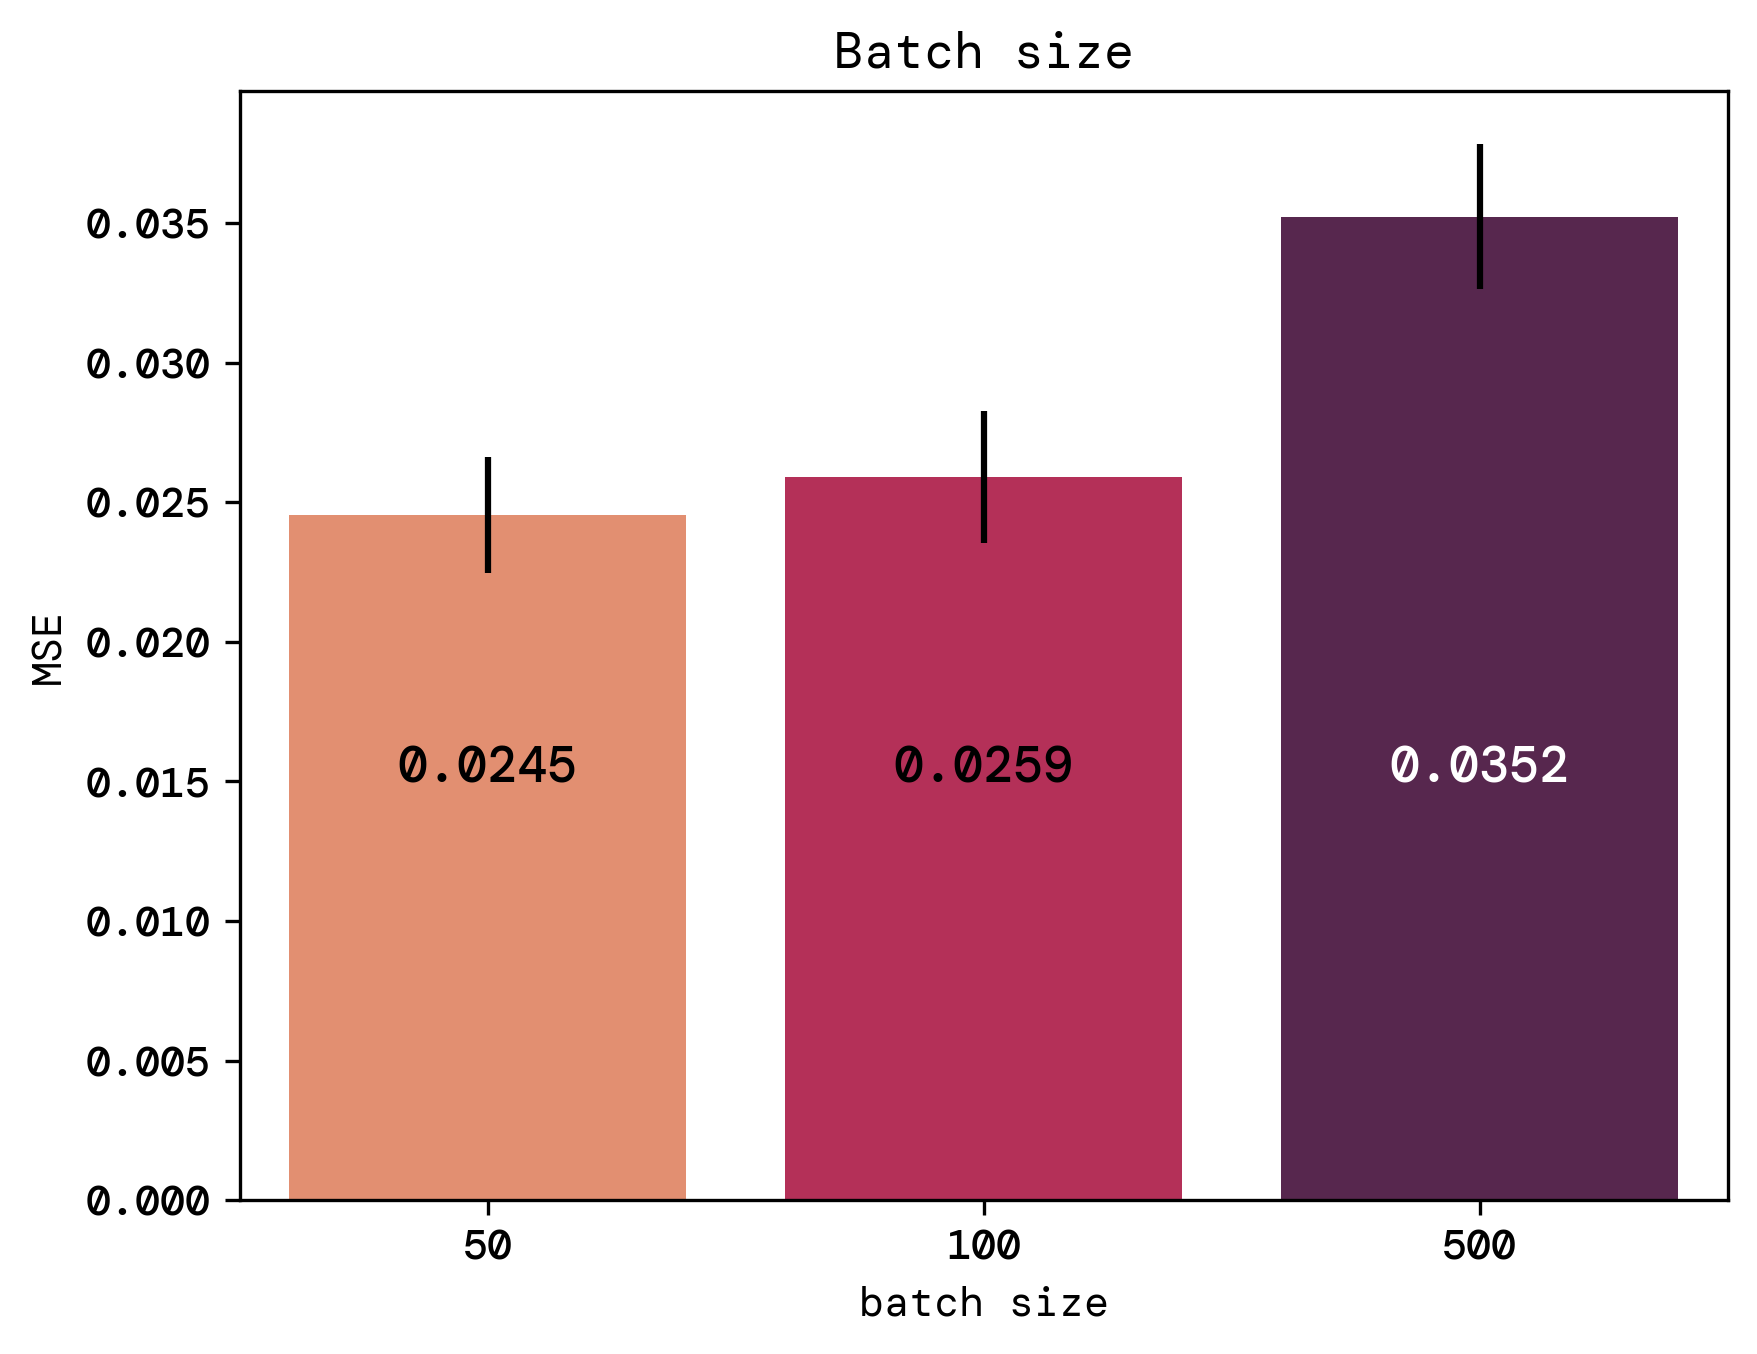
\includegraphics[width=\textwidth]{../runsAndFigures/MSE_batch.png}
            \end{center}
            \caption{Introduction regualarization does not seem to yield any benefits, in fact
            having too much regualarization shunts performance}\label{fig:MSE_batch}
        \end{minipage}
    \end{figure}

    \begin{figure}[!ht]
        \begin{minipage}[t]{0.5\textwidth - 1mm}
            \begin{center}
                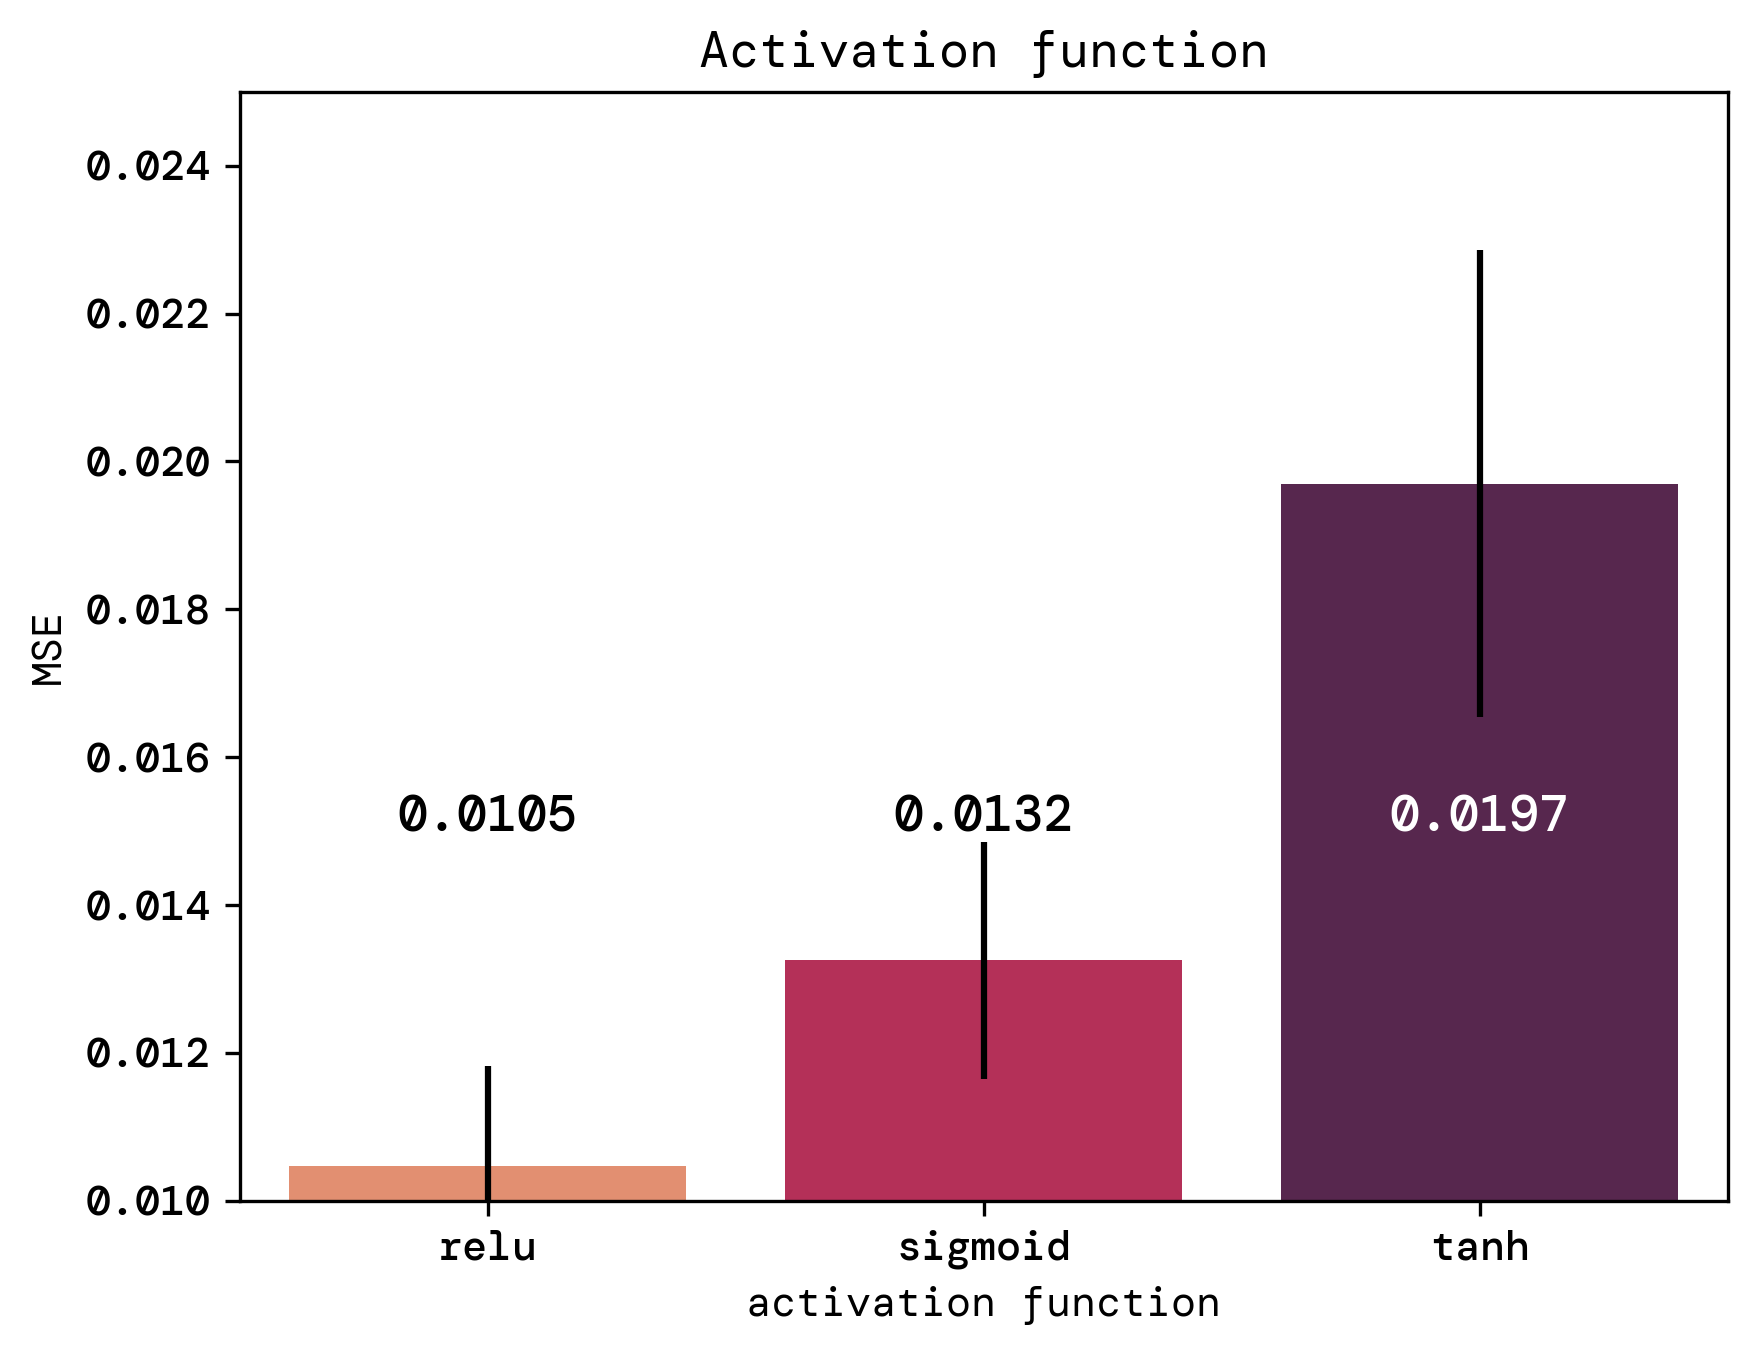
\includegraphics[width=\textwidth]{../runsAndFigures/MSE_activs.png}
            \end{center}
            \caption{In this case havving momentum seems to be beneficial.
            We maxes out our testing range and found that 0.9 was the best value for momentum. 
            momentum allows a higher learning rate}\label{fig:accuracy_optimizer}
        \end{minipage}
        \hspace{2mm}
        \begin{minipage}[t]{0.5\textwidth - 1mm}
            \begin{center}
                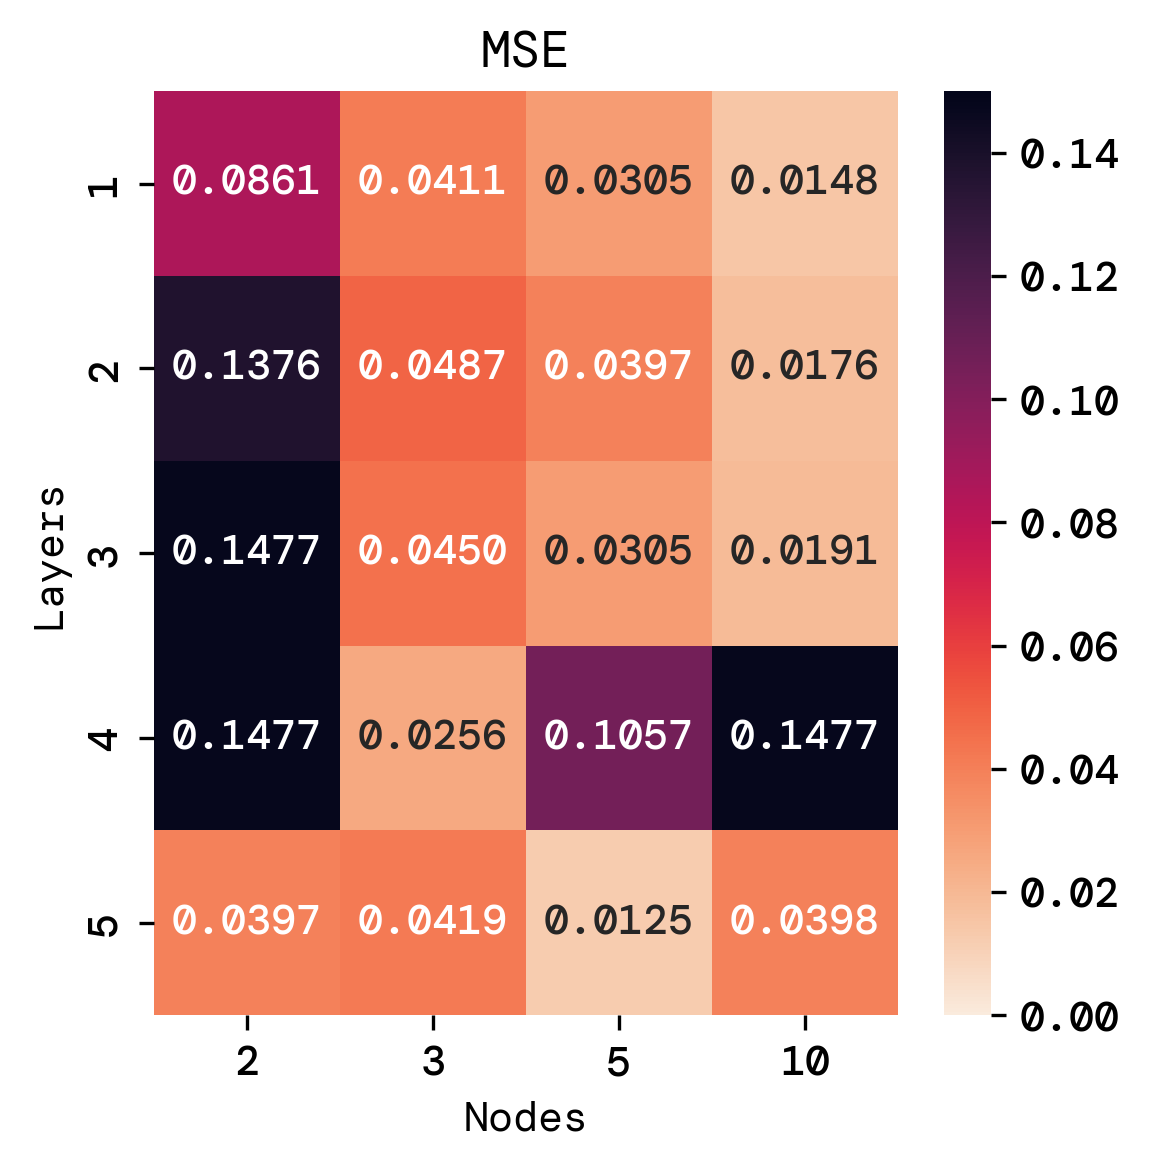
\includegraphics[width=\textwidth]{../runsAndFigures/MSE_layers_nodes.png}
            \end{center}
            \caption{Introduction regualarization does not seem to yield any benefits, in fact
            having too much regualarization shunts performance}\label{fig:accuracy_aplha}
        \end{minipage}
    \end{figure}


    \begin{figure}
        \begin{center}
            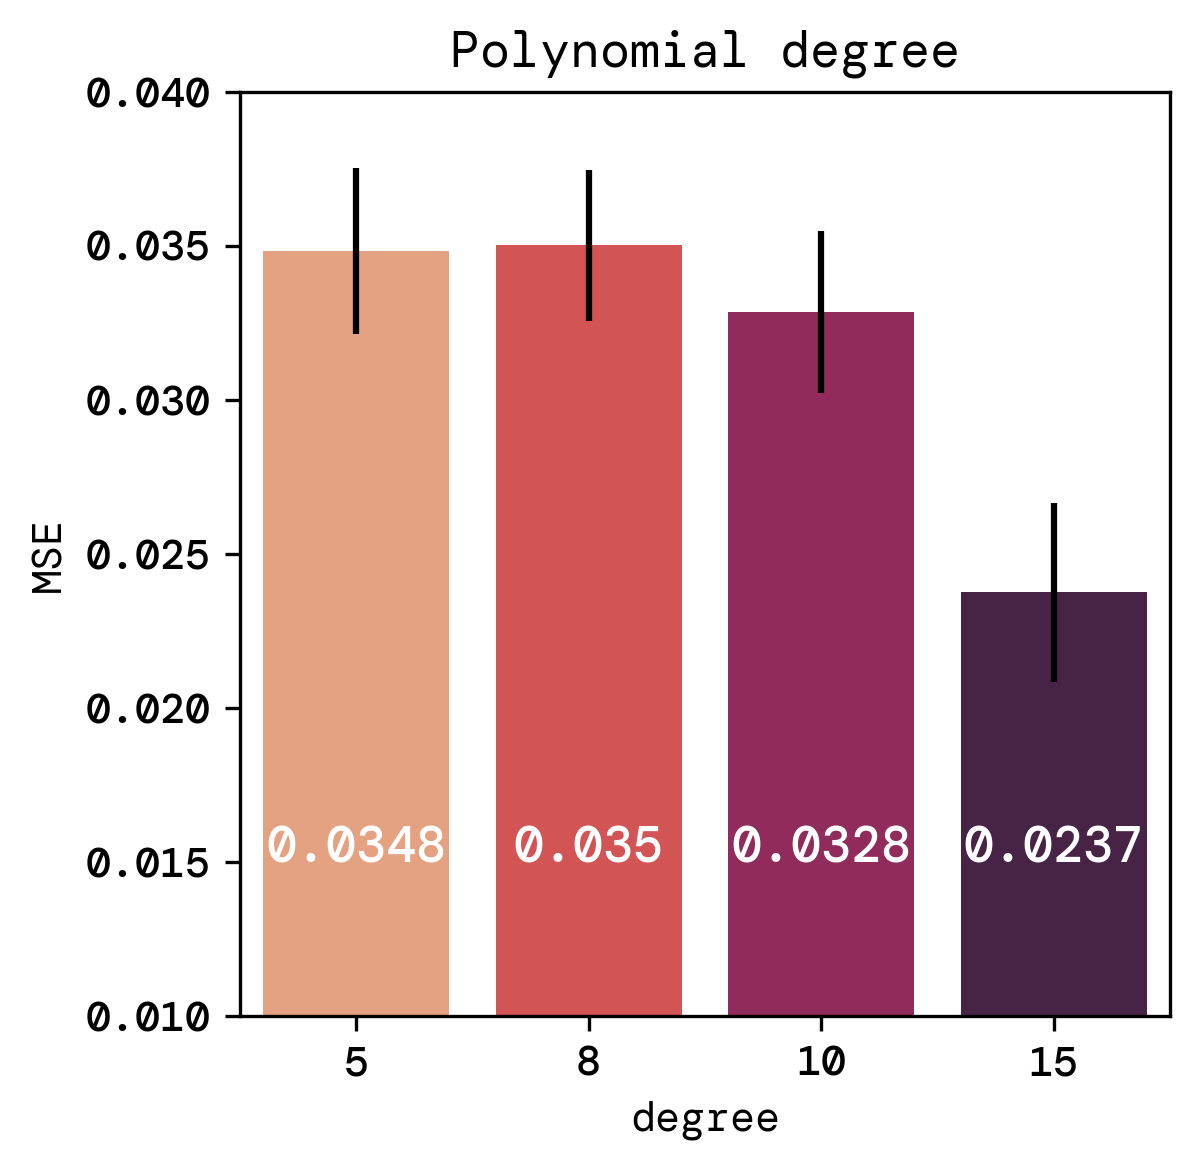
\includegraphics[width=0.95\textwidth]{../runsAndFigures/MSE_degree.png}
        \end{center}
        \caption{}\label{fig:}
    \end{figure}



\subsection*{Final Evaluation and Comparisons}
\label{sec:comparisons2}






    \begin{figure}[!ht]
        \begin{minipage}[t]{0.5\textwidth - 1mm}
            \begin{center}
                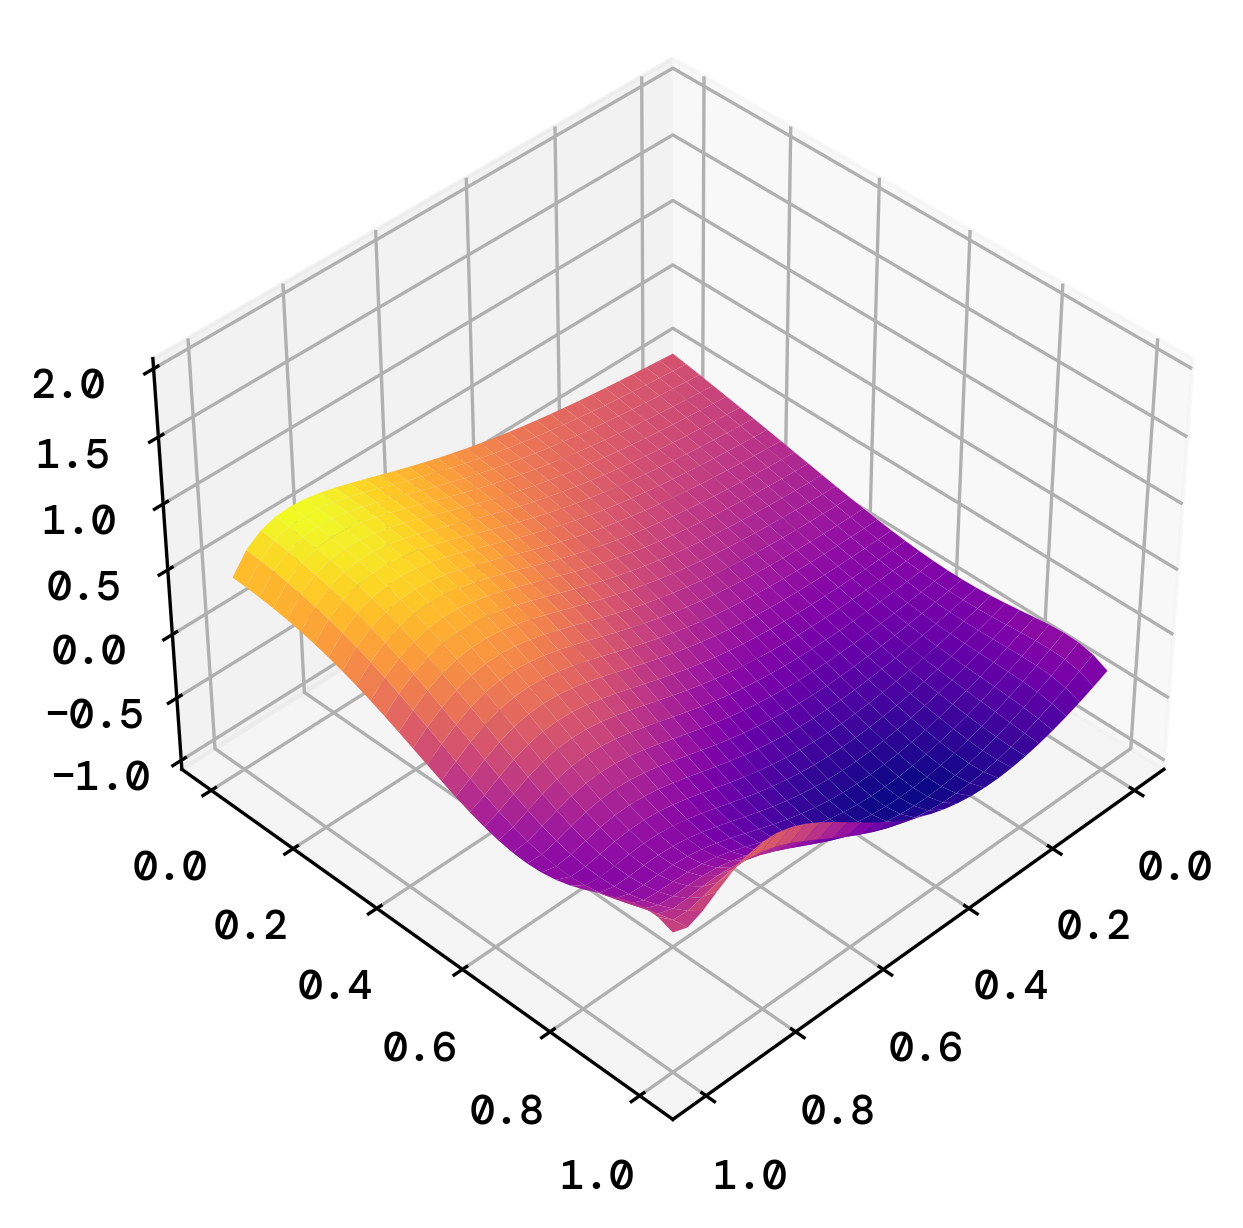
\includegraphics[width=\textwidth]{../runsAndFigures/perlinNoise_logistic_pred.png}
            \end{center}
            \caption{In this case havving momentum seems to be beneficial. We maxes out our testing range 
            and found that 0.9 was the best value for momentum. momentum allows a higher learning rate
        }\label{fig:accuracy_optimizer}
        \end{minipage}
        \hspace{2mm}
        \begin{minipage}[t]{0.5\textwidth - 1mm}
            \begin{center}
                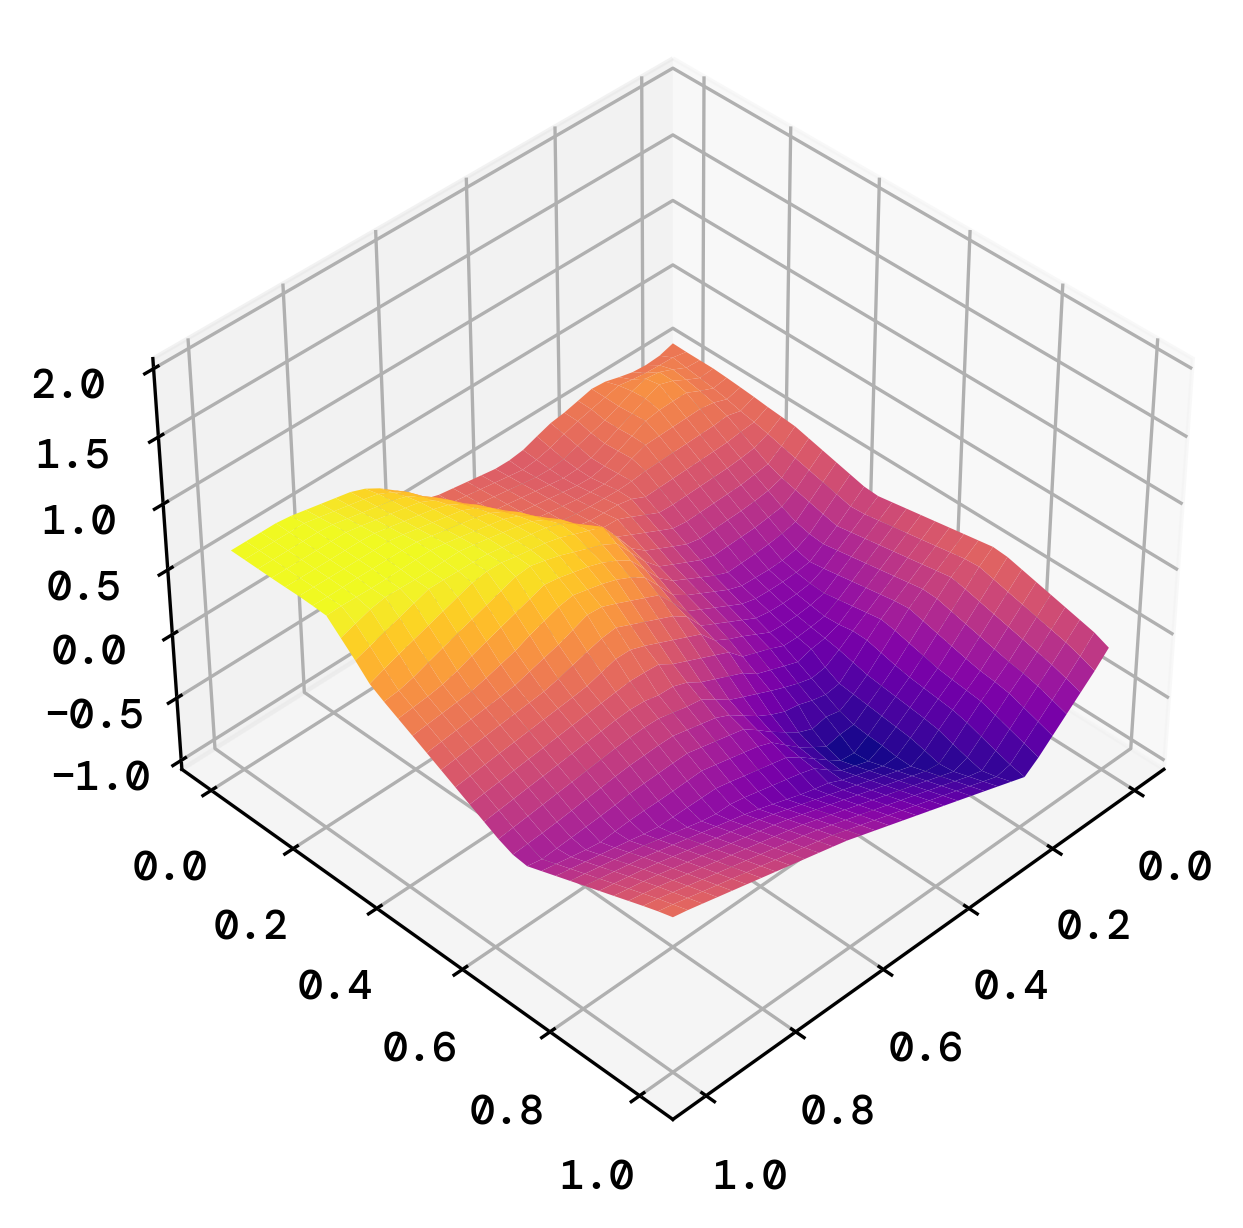
\includegraphics[width=\textwidth]{../runsAndFigures/perlinNoise_NN_pred.png}
            \end{center}
            \caption{Introduction regualarization does not seem to yield any benefits, in fact
            having too much regualarization shunts performance}\label{fig:accuracy_aplha}
        \end{minipage}
    \end{figure}











\chapter*{Appendix B}
\label{app:appendixB}


\section{Universal Approximation}
\label{sec:UAT}

    Where is the limit of what we can learn with a neural network? Can we approximate any function?
    There are several ways to approximate a function. For periodic functions it may be wise to use a Fourier series,
    another option is to use a Taylor series. If these mehtods don't float your boat, we can in fact use a neural network
    instead. A neural network with only one hidden layer can approximate any continuous function
    given enough neurons in the hidden layer. The more neurons, the higher the resolution of the Approximation
    \cite{HornikEtAl89}. 

\subsection*{XOR VS Perceptron}
\label{app:xor}

    \begin{wrapfigure}{r}{0.5\textwidth}
        \begin{center}
            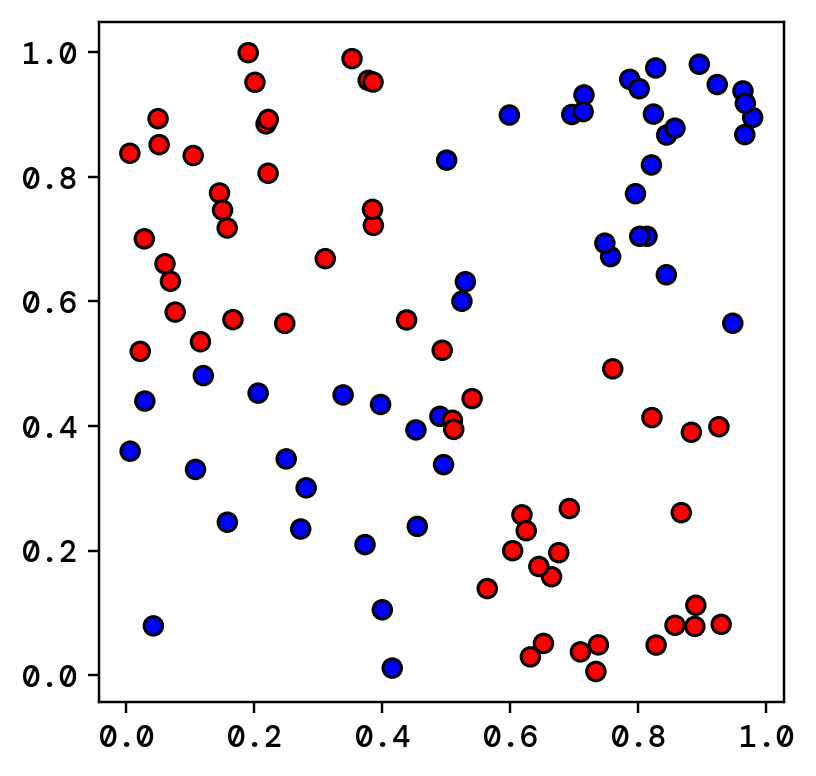
\includegraphics[width=0.4\textwidth]{../runsAndFigures/xor.png}
        \end{center}
        \caption{}\label{fig:xor_data}
    \end{wrapfigure}

    A perceptron is a simple model of a neuron. It takes in a set of inputs, multiplies them by a set of weights 
    and sums them up to produce an output. The output is then passed through the heaviside
    \footnote{We use sigmoid instead of the heaviside, but the outcome of the classification is the same.}
    step function to produce
    a binary output. The perceptron can be used to solve simple classification problems. However, it is not able to
    solve the XOR problem. XOR is not linearly separable, meaning that it is not possible to draw a straight line
    that separates the two classes. This is a problem for the perceptron, as it can only draw straight lines.
    One way to solve this problem is to add some polynomial features to the data. 
    This will allow us to draw a curved line that separates the two classes. However, this is not a scalable solution.
    NNs can also learn xor, without the need for a polynomial feature. This is important because it is not 
    always obvious what feature engineering is required to solve a problem. Neural networks can learn the 
    relevant 
    features from the data. Manually adding polynomial features is not a scalable solution for 
    high-dimensional data,
    whereas neural networks can learn arbitrarily complex functions. Adding polynomial featurer 
    is also prone to 
    bias problems.




    \begin{figure}[h]
        \begin{minipage}{0.5\textwidth - 1mm}
            \begin{center}
                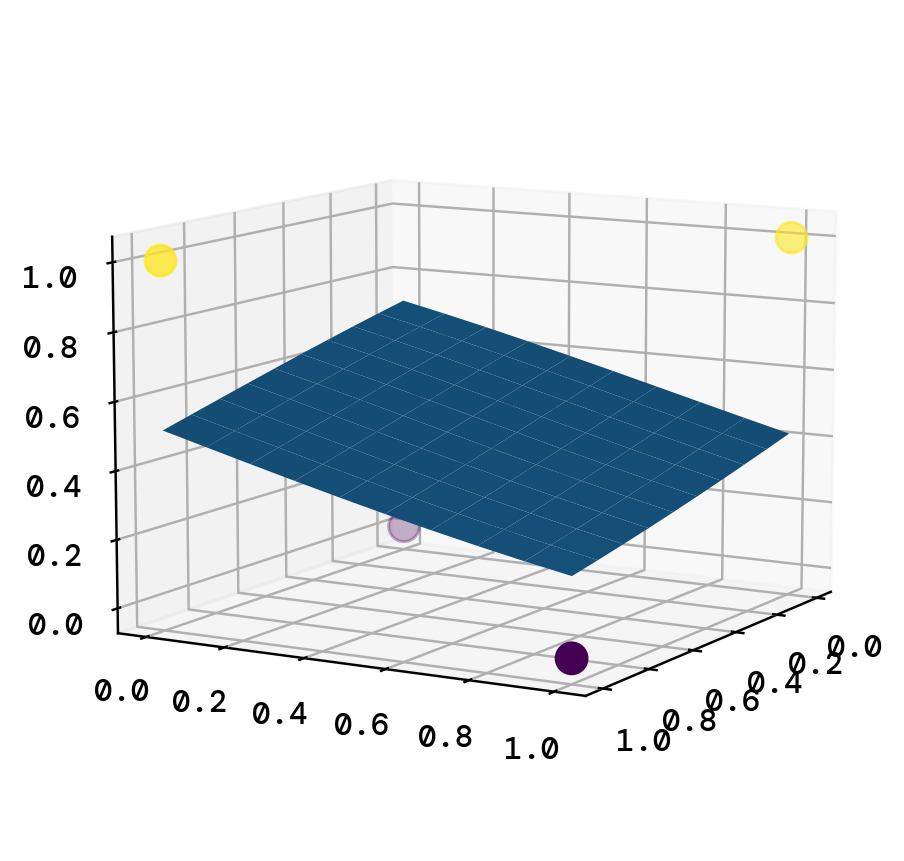
\includegraphics[width=\textwidth]{../runsAndFigures/xor_plain.png}
                \caption{}\label{fig:xor_plain}
            \end{center}
        \end{minipage}
        \hspace{2mm}
        \begin{minipage}{0.5\textwidth - 1mm}
            \begin{center}
                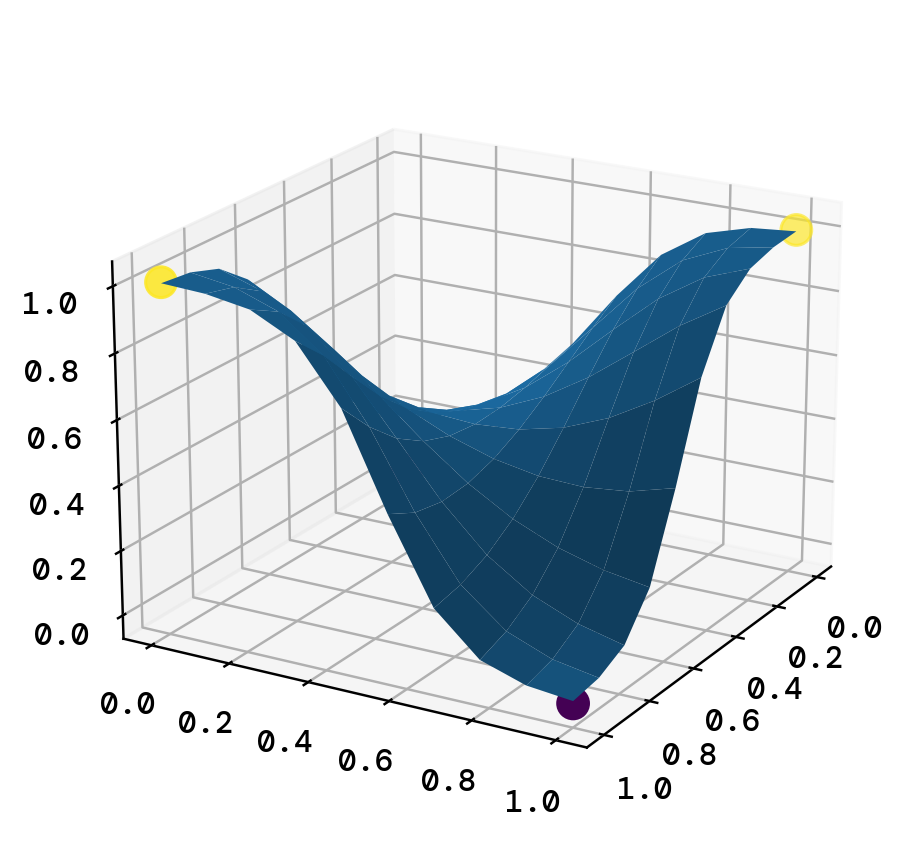
\includegraphics[width=\textwidth]{../runsAndFigures/xor_poly.png}
                \caption{}\label{fig:xor_poly}
            \end{center}
        \end{minipage}
    \end{figure}



    \begin{figure}[!h]
        \begin{center}
            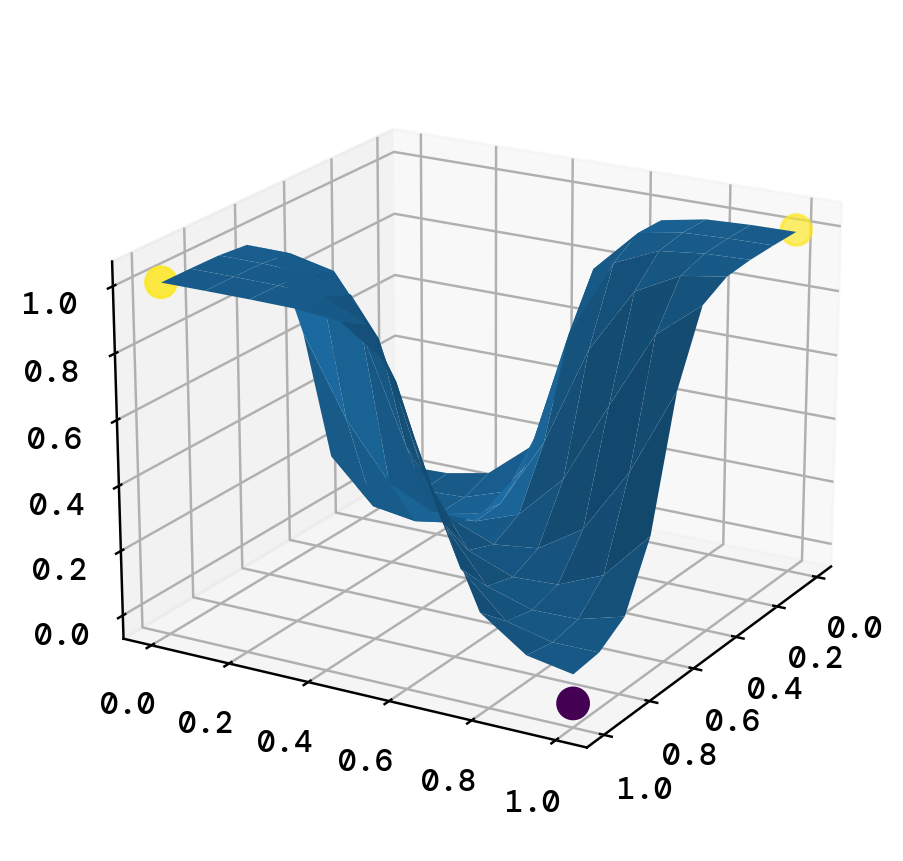
\includegraphics[width=0.5\textwidth]{../runsAndFigures/xor_nn.png}
        \end{center}
        \caption{}\label{fig:xor_nn}
    \end{figure}



\subsection*{Combining Neurons}
\label{app:neuronscombined}

    We want to approximate this sin function with a neural network. How might that look like?
    We can use a single neuron to approximate a line $a w + b$, putting it trough a sigmoid function
    we get some non-linearity. Every node in the first hidden layer (and consequents layers) is then 
    a line put trough a sigmoid function. The final output of a single hidden layer network is just
    a linear combination of these curves. We can add more nodes to get more curves, but we are still
    We can chose whatever activation function we want as long as it is non-linear. Relu strugles to learn this 
    sin function, but sigmoid works fine.


    \begin{figure}
        \begin{center}
            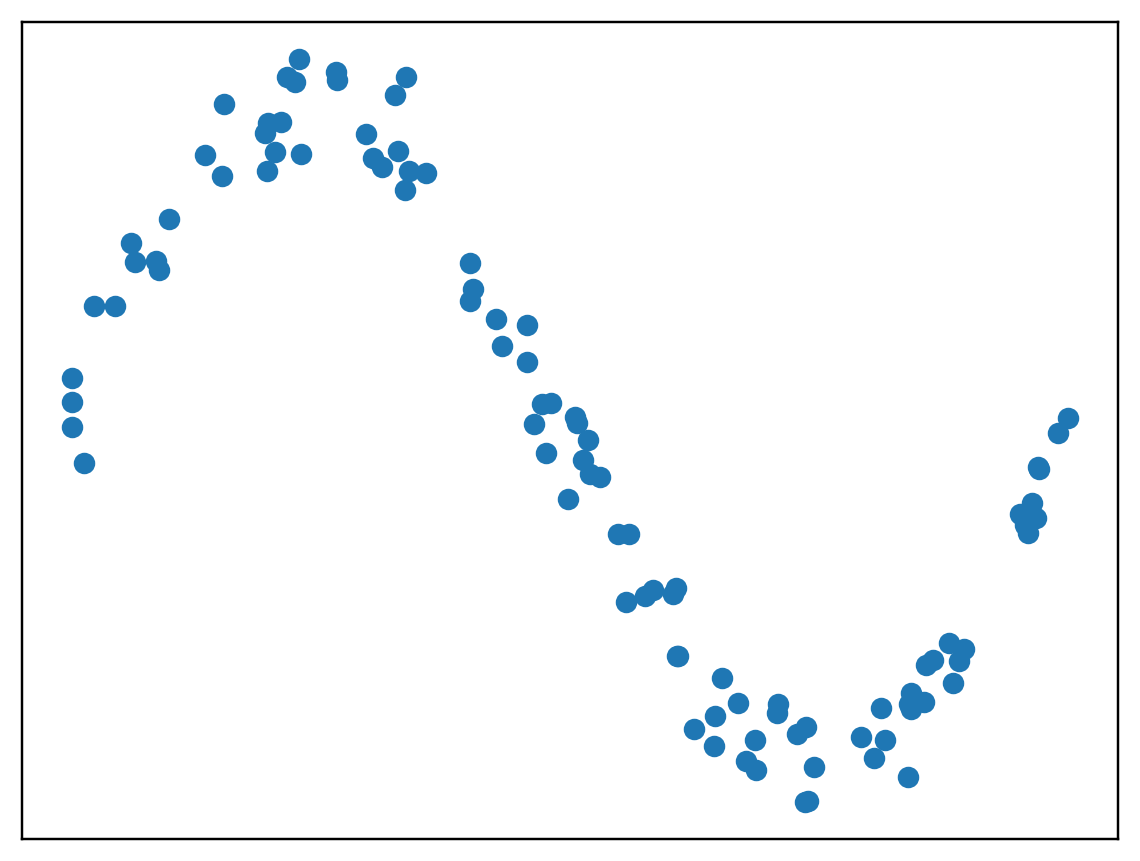
\includegraphics[width=0.4\textwidth]{../runsAndFigures/sin.png}
        \end{center}
        \caption{A $\text{sin}$ function that we want to approximate}\label{fig:sin}
    \end{figure}

    \begin{figure}
        \begin{center}
            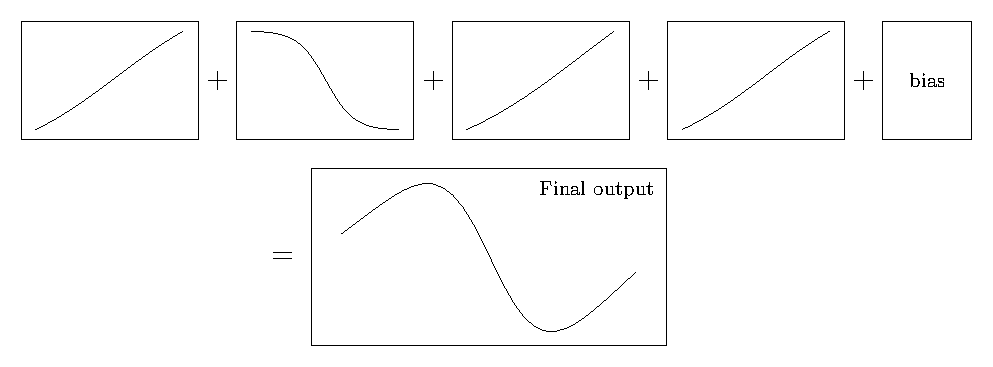
\includegraphics[width=0.95\textwidth]{tikzfigures/universal.pdf}
        \end{center}
        \caption{Four indivudual logistic regression outputs scaled and added together to produce 
        a sin approximation}\label{fig:universal}
    \end{figure}






\vskip 0.2in
\bibliography{report}
% \bibliographystyle{apalike}
\bibliographystyle{plain}
\addcontentsline{toc}{section}{Bibliography}
\end{document}

